\chapter{Couplage électron-défaut dans le graphène}\label{chap:défauts}

Ce chapitre se consacre au couplage entre les électrons et les défauts, l'un des ingrédients essentiels au calcul de l'intensité Raman résonante des processus \textit{phonon-défaut} introduits au chapitre~\ref{chap:Raman}, et constitue le c\oe ur des contributions originales de ce mémoire. Le couplage entre les électrons et les défauts intervient à deux endroits dans la théorie : directement, par les éléments de matrice $M_{mn}(\kv',\kv)$ qui apparaissent dans les amplitudes de diffusion \textit{phonon-défaut}, et indirectement, par le taux d'amortissement $\Gamma_{n\kv}^\text{ed}$, qui renormalise les temps de vie électroniques. Nous commençons par définir la matrice $\bm M$, dérivons comment la calculer à partir des premiers principes, montrons comment l'interpoler sur des grilles denses grâce aux fonctions de Wannier et la calculons pour une lacune dans le graphène. Les observables physiques qui en découlent sont calculées avec la théorie de la perturbation à plusieurs corps dans le chapitre suivant.

Contrairement au couplage électron-phonon, pour lequel la communauté dispose d'un cadre théorique mûr~\cite{giustinoElectronphononInteractionsFirst2017,giustinoElectronphononInteractionUsing2007} et d'outils standards implémentés dans des codes largement distribués~\cite{ponceEPWElectronphononCoupling2016,leeElectronPhononPhysics2023a,zhouPerturboSoftwarePackage2021,gonzeAbinitProjectImpact2020,bruninPhononlimitedElectronMobility2020}, le calcul \textit{ab initio} du couplage électron-défaut en est encore à ses débuts. Aucun code communautaire n'en fait une quantité de routine et les rares études existantes reposent sur des implémentations dédiées ou bien ne traitent pas les défauts à partir des premiers principes (par exemple, Venezuela \textit{et al.}~\cite{venezuelaTheoryDoubleresonantRaman2011} simulent l'intensité Raman résonante du graphène avec des défauts, mais les modélisent avec un modèle de liaisons fortes). Lu, Zhou et Bernardi ont développé le calcul des éléments de matrice électron-défaut en ondes planes~\cite{luEfficientInitioCalculations2019} et leur interpolation par fonctions de Wannier~\cite{luInitioElectrondefectInteractions2020}, dont ce chapitre s'inspire, mais traitent la diffusion dans l'approximation de Born, insuffisante pour les défauts à potentiel fort de ce mémoire. Kaasbjerg~\cite{kaasbjergAtomisticMatrixTheory2020} traite au contraire la diffusion à tous les ordres par la matrice $T$, mais le fait dans une base d'orbitales atomiques localisées dont la convergence systématique ne se contrôle pas. Ce chapitre et le suivant combinent les deux approches. Dans celui-ci, la matrice de couplage est calculée \textit{ab initio} en ondes planes, raffinée par un remplissage par zéros, puis interpolée par fonctions de Wannier. Dans le suivant, la matrice $T$ est résolue en exploitant sa localisation dans l'espace, rendue manifeste par les fonctions de Wannier, à faible coût numérique sur des grilles arbitrairement denses.

\section{Éléments de matrice électron-défaut}\label{sec:M_défaut}

L'élément central à l'étude de défauts dans un matériau à partir des premiers principes est la matrice de couplage électron-défaut
\begin{equation}
    M_{mn}(\kv',\kv) = \matrixel{\psi_{m\kv'}}{V_\text{ed}(\rv)}{\psi_{n\kv}},\label{eqn:M}
\end{equation}
qui correspond physiquement à l'amplitude de probabilité que l'électron dans l'état $n\kv$ diffuse vers l'état $m\kv'$ à cause du potentiel $V_\text{ed}(\rv)$ induit par le défaut dans le matériau. L'Hamiltonien associé à ce couplage est donné par
\begin{equation}
    \hat{H}_\text{ed} = \frac{1}{N_\text{uc}}\sum_{mn}\sum_{\kv\kv'}M_{mn}(\kv',\kv)\hat{c}^\dag_{m\kv'}\hat{c}_{n\kv},
\end{equation}
écrit en deuxième quantification. Pour ce qui suit, $\bm M$ en gras désigne la matrice complète dans l'indice composé $n\kv$ (ou $i\Rv$ dans la base de Wannier) et $M_{mn}(\kv',\kv)$ ses éléments. Cet Hamiltonien est inclus perturbativement dans le terme d'interaction de l'Hamiltonien complet et la matrice de couplage peut être vue comme l'élément de matrice de la perturbation $V_\text{ed}(\rv)$ au premier ordre dans la base des états non perturbés. Cette approche est valide pour des potentiels de défauts faibles. Toutefois, les défauts usuels, comme les lacunes, les substitutions ou les adatomes, induisent des potentiels qui ne sont généralement pas faibles~\cite{banhartStructuralDefectsGraphene2011}, et un traitement au premier ordre est insuffisant. Nous verrons au chapitre~\ref{chap:T} que la théorie de la perturbation à plusieurs corps permet de sommer les corrections à tous les ordres, pour un seul défaut, ce qui rend le traitement valable quelle que soit la force du potentiel de défaut.

La présence d'un ou plusieurs défauts dans un matériau brise explicitement la symétrie de translation discrète et la périodicité du cristal : le théorème de Bloch ne s'applique plus, ce qui complique fortement l'étude des défauts \textit{ab initio}. Pour contourner ces difficultés, il est utile de placer le défaut au centre d'une \textit{super-cellule}~\cite{freysoldtFirstprinciplesCalculationsPoint2014}, c'est-à-dire une répétition de $N_\text{cells} = N\times N$ (en deux dimensions, à ne pas confondre avec $N_\text{uc}$ qui dénote le nombre de cellules unitaires dans tout le cristal) cellules unitaires et de résoudre le problème électronique pour deux super-cellules : une contenant le défaut, appelée la super-cellule \textit{défectueuse}, et une ne contenant pas de défaut, appelée la super-cellule \textit{parfaite}. Une fois le problème résolu avec la DFT pour les deux super-cellules, nous avons les potentiels de Kohn-Sham convergés de la super-cellule défectueuse $V_\text{KS}^\text{d}(\rv)$ et de la super-cellule parfaite $V_\text{KS}^\text{p}(\rv)$ et le potentiel induit par le défaut est défini comme étant la différence des deux
\begin{equation}
    V_\text{ed}(\rv) = V_\text{KS}^\text{d}(\rv) - V_\text{KS}^\text{p}(\rv).\label{eqn:V_ed}
\end{equation}
Il est critique que la super-cellule soit assez grande pour contenir le défaut, c'est-à-dire que $V_\text{ed}(\rv)$ soit négligeable à ses frontières. Cela garantit que le défaut n'interagit pas avec ses images périodiques artificielles.

Pour un défaut neutre, le potentiel est de courte portée et une super-cellule de taille modeste suffit à le contenir. Les défauts chargés font exception : la queue coulombienne de leur potentiel, en $1/r$, exige des super-cellules bien plus grandes ou un traitement séparé de la partie de longue portée~\cite{freysoldtFullyInitioFiniteSize2009,luFirstprinciplesIonizedimpurityScattering2021}. Nous ne considérons dans ce mémoire qu'une lacune neutre, c'est-à-dire un atome manquant dans le réseau cristallin, dont le potentiel est de courte portée mais très intense près du défaut.

Nous avons vu dans la section~\ref{sec:PP} que le potentiel de Kohn-Sham se décompose en une partie locale et une partie non locale due aux pseudo-potentiels. De manière similaire, le potentiel de défaut se sépare en deux parties
\begin{equation}
    V_\text{ed}(\rv) = V_\text{ed}^\text{L}(\rv)+\hat{V}_\text{ed}^\text{NL}.
\end{equation}
La partie locale est donnée par la somme des potentiels d'Hartree, d'échange-corrélation et de la partie locale du pseudo-potentiel
\begin{equation}
    V^\text{x,L}(\rv) = V_\text{H}^\text{x}(\rv) + V_\text{XC}^\text{x}(\rv)+V_\text{PPL}^\text{x}(\rv),
\end{equation}
où $\text{x} = \text{d},\text{p}$ et la partie non locale est due entièrement aux parties non locales des pseudo-potentiels
\begin{equation}
    \hat{V}^\text{x,NL} = \sum_{\alpha}\sum_{i\ell m_\ell}\ket{\beta_{i\ell m_\ell}^{\text{x}(\alpha)}}E_{i\ell}^{\text{x}(\alpha)}\bra{\beta_{i\ell m_\ell}^{\text{x}(\alpha)}}.\label{eqn:V_ed_NL}
\end{equation}
Les parties locale et non locale du potentiel de défaut s'obtiennent par la même soustraction que le potentiel total~\eqref{eqn:V_ed}, soit $V_\text{ed}^\text{L} = V^\text{d,L}-V^\text{p,L}$ et $\hat{V}_\text{ed}^\text{NL} = \hat{V}^\text{d,NL}-\hat{V}^\text{p,NL}$, l'indice \og ed \fg{} étant réservé aux différences. Par conséquent, la matrice de couplage électron-défaut se sépare aussi en une partie locale et une partie non locale
\begin{equation}
    M_{mn}(\kv',\kv) = M_{mn}^\text{L}(\kv',\kv) + M_{mn}^\text{NL}(\kv',\kv).
\end{equation}
Ces deux parties sont calculées indépendamment, puis additionnées pour retrouver la matrice de couplage totale. Nous voyons maintenant comment calculer ces deux parties.

\section{Partie locale}\label{sec:M_local}

Commençons par dériver une expression pour la partie locale de la matrice. Cette dérivation suit l'approche de Lu, Zhou et Bernardi~\cite{luEfficientInitioCalculations2019}. Premièrement, dans l'espace réel, la partie locale est
\begin{equation}
    M^\text{L}_{mn}(\kv',\kv) = \matrixel{\psi_{m\kv'}}{V_\text{ed}^\text{L}(\rv)}{\psi_{n\kv}} = \int_{\Omega_\text{BvK}}d^3\rv\,\psi_{m\kv'}^*(\rv)\,V^\text{L}_\text{ed}(\rv)\,\psi_{n\kv}(\rv),\label{eqn:ML_réel}
\end{equation}
où l'intégration se fait sur le volume du cristal $\Omega_\text{BvK}$. Le potentiel $V_\text{ed}^\text{L}(\rv)$ est défini sur la grille de la super-cellule, tandis que les états $\ket{\psi_{n\kv}}$ sont les états propres sur la grille de la cellule unitaire parfaite. Pour évaluer l'intégrande, ces états de Bloch doivent être échantillonnés sur la même grille que le potentiel $V_\text{ed}^\text{L}(\rv)$, c'est-à-dire celle de la super-cellule. Évaluer cette intégrale directement dans l'espace réel exigerait de représenter chaque état de Bloch sur cette grille, au prix d'une empreinte en mémoire qui devient vite rédhibitoire à mesure que la super-cellule grandit. Il est plus efficace de passer à l'espace réciproque où les états de Bloch sont décrits par leurs coefficients d'ondes planes dans la cellule unitaire du cristal parfait et la super-cellule n'intervient qu'à travers ses composantes de Fourier. Le coût en mémoire est ainsi découplé de la taille de la super-cellule, qui ne détermine plus que la résolution du potentiel dans l'espace réciproque.

Ce potentiel est celui d'une lacune isolée dans le cristal : il ne possède pas la périodicité de la super-cellule. Pour passer à l'espace réciproque, nous le développons en série de Fourier sur tous les vecteurs d'onde $\qv+\Gv$ permis par les conditions aux frontières de Born--von Kármán, où $\qv$ parcourt les $N_\text{uc}$ points de la grille du cristal entier dans sa première zone de Brillouin et $\Gv$ parcourt ceux du réseau réciproque de la cellule unitaire
\begin{equation}
    V_\text{ed}^\text{L}(\rv) = \frac{1}{N_\text{uc}}\sum_{\qv}\sum_{\Gv}\widetilde{V}_\text{ed}^\text{L}(\qv+\Gv)e^{i(\qv+\Gv)\cdot\rv},
\end{equation}
où $N_\text{uc}$ est le nombre de cellules unitaires dans le cristal (de sorte que $\Omega_\text{BvK}=N_\text{uc}\Omega_\text{uc}$). Sa transformée de Fourier inverse est définie comme étant
\begin{align}
    \widetilde{V}_\text{ed}^\text{L}(\qv+\Gv) &= \frac{1}{\Omega_\text{uc}}\int_{\Omega_\text{BvK}}d^3\rv\,V_\text{ed}^\text{L}(\rv)e^{-i(\qv+\Gv)\cdot\rv},\\
    &\approx \frac{1}{\Omega_\text{uc}}\int_{\Omega_\text{sc}}d^3\rv\,V_\text{ed}^\text{L}(\rv)e^{-i(\qv+\Gv)\cdot\rv},
\end{align}
où l'intégrale sur le cristal se réduit à une intégrale sur une super-cellule puisque le potentiel, une fois sa référence fixée, est négligeable aux frontières de celle-ci. Pour les fonctions d'onde de la cellule unitaire, nous utilisons leur forme donnée par le théorème de Bloch~\eqref{eqn:c2_bloch_thm}, ce qui donne
\begin{equation}
    M^\text{L}_{mn}(\kv',\kv) = \frac{1}{N_\text{uc}}\sum_{\qv}\sum_\Gv\widetilde{V}_\text{ed}^\text{L}(\qv+\Gv)\int_{\Omega_\text{BvK}}d^3\rv\,u^*_{m\kv'}(\rv)\,u_{n\kv}(\rv)\,e^{i(\kv+\qv+\Gv-\kv')\cdot\rv}.
\end{equation}
Ensuite, nous utilisons l'invariance des parties périodiques de Bloch sous une translation d'un vecteur du réseau $\Rv$ du système parfait pour décomposer l'intégrale sur le cristal comme une somme d'intégrales sur une cellule unitaire
\begin{equation}
    M^\text{L}_{mn}(\kv',\kv) = \frac{1}{N_\text{uc}}\sum_{\qv}\sum_\Gv\widetilde{V}_\text{ed}^\text{L}(\qv+\Gv)\sum_\Rv e^{i(\kv+\qv+\Gv-\kv')\cdot\Rv}\int_{\Omega_\text{uc}} d^3\rv\,u_{m\kv'}^*(\rv)\,u_{n\kv}(\rv)e^{i(\kv+\qv+\Gv-\kv')\cdot\rv}.
\end{equation}
Comme $e^{i\Gv\cdot\Rv}=1$, la somme sur $\Rv$ ne dépend que de $\qv$ : elle vaut $N_\text{uc}$ pour le seul point $\qv=\kv'-\kv+\Gv_0$ de la grille, où $\Gv_0$ est le vecteur du réseau réciproque qui ramène $\kv'-\kv$ dans la première zone de Brillouin, et zéro ailleurs. La somme sur $\qv$ se réduit à ce terme et le facteur $N_\text{uc}$ compense $1/N_\text{uc}$
\begin{equation}
    M^\text{L}_{mn}(\kv',\kv) = \sum_{\Gv}\widetilde{V}_\text{ed}^\text{L}(\kv'-\kv+ \Gv_0 + \Gv)\int_{\Omega_\text{uc}} d^3\rv\,u_{m\kv'}^*(\rv)\,u_{n\kv}(\rv)e^{i(\Gv_0 + \Gv)\cdot\rv}.
\end{equation}
Puisque la somme court sur tous les vecteurs $\Gv$, le changement d'indice $\Gv+\Gv_0\to\Gv$ élimine $\Gv_0$. Ensuite, en définissant le transfert de quantité de mouvement $\qv\equiv\kv'-\kv$ et en utilisant le développement de la partie périodique de Bloch en ondes planes~\eqref{eqn:c2_uPW}, nous obtenons
\begin{equation}
     M^\text{L}_{mn}(\kv',\kv) = \frac{1}{\Omega_\text{uc}}\sum_{\Gv\Gv'\Gv''}\widetilde{V}_\text{ed}^\text{L}(\qv+\Gv)C_{m\kv'}^*(\Gv')C_{n\kv}(\Gv'')\underbrace{\int_{\Omega_\text{uc}} d^3\rv\,e^{i(\Gv+\Gv''-\Gv')\cdot\rv}}_{=\Omega_\text{uc}\delta_{\Gv+\Gv'',\Gv'}}.
\end{equation}
Enfin, en effectuant la somme sur $\Gv'$, nous obtenons l'équation pratique que nous avons implémentée pour calculer la partie locale de la matrice de couplage électron-défaut
\begin{equation}
    M_{mn}^\text{L}(\kv',\kv) = \sum_{\Gv\Gv''}\widetilde{V}_\text{ed}^\text{L}(\qv+\Gv)C_{m\kv'}^*(\Gv+\Gv'')C_{n\kv}(\Gv'').\label{eqn:ML_final}
\end{equation}
L'évaluation de l'équation~\eqref{eqn:ML_final} requiert la composante de Fourier $\widetilde{V}_\text{ed}^\text{L}(\qv+\Gv)$ du défaut isolé pour chaque transfert $\qv$ de la cellule unitaire. Or, un calcul de super-cellule ne fournit que les composantes de Fourier du potentiel sur le réseau réciproque de cette dernière. Ce réseau réciproque contient celui de la cellule unitaire de sorte que la composante requise est disponible si $\qv$ est lui-même un point de la grille de la super-cellule. Ceci est automatiquement satisfait si la grille de la cellule unitaire est commensurable avec celle de la super-cellule.

En pratique, nous effectuons les calculs de super-cellule au seul point $\Gamma$ d'une super-cellule $N\times N$. Le potentiel $\widetilde{V}_\text{ed}^\text{L}$ n'est alors connu que sur les vecteurs $\widetilde{\Gv}$ du réseau réciproque de celle-ci, espacés de $1/N$ (en unités du réseau réciproque de la cellule unitaire). Pour que le transfert $\qv=\kv'-\kv$ requis dans l'équation~\eqref{eqn:ML_final} coïncide avec l'un de ces vecteurs, la grille de la cellule unitaire doit être commensurable avec la super-cellule : une grille $m\times m$ convient si et seulement si $m$ divise $N$. Ainsi, à titre d'exemple, une super-cellule $10\times 10$ (à $\Gamma$) autorise seulement les grilles $5\times 5$ et $10\times 10$ (et les grilles triviales $1\times 1$ et $2\times 2$) pour la cellule unitaire.

Cette contrainte est très restrictive. La taille de la super-cellule est dictée par la physique du défaut : elle doit être suffisamment grande pour que le potentiel, une fois sa référence fixée, soit négligeable aux frontières. Cependant, pour se prêter à l'interpolation par fonctions de Wannier, la grille de la cellule unitaire doit être celle des fonctions de Wannier. Imposer la commensurabilité forcerait alors des super-cellules inutilement grandes, au prix d'un coût de calcul prohibitif. À titre d'illustration, pour utiliser les fonctions de Wannier sur la grille $27\times 27$ de la section~\ref{sec:electron_results}, il faut une super-cellule $27\times 27$ qui contient, pour le graphène, 1458 atomes de carbone et 5832 électrons de valence. Cette situation s'accentue d'autant plus pour la plupart des autres matériaux, qui contiennent généralement plus de deux atomes dans leur cellule unitaire.

Face à ce coût computationnel substantiel, nous contournons cette contrainte en raffinant la grille du potentiel par remplissage par zéros (\textit{zero padding}). Si la lacune est isolée et localisée, et si nous supposons que son potentiel est nul loin de celle-ci, compléter le potentiel par des zéros dans une boîte plus grande le reproduit exactement. La transformée de Fourier de ce potentiel élargi fournit alors ses composantes de Fourier sur une grille plus dense, pouvant contenir tous les transferts de la grille unitaire désirée. En vertu du théorème d'échantillonnage, cette opération est \textit{exacte} et non approximative~\cite{shannonCommunicationPresenceNoise1949} : un potentiel qui s'annule \textit{exactement} hors d'une région finie de l'espace est entièrement déterminé par ses composantes de Fourier sur la grille de la super-cellule et les transferts intermédiaires s'en déduisent sans perte d'information. Il y a toutefois deux réserves. D'abord, si le potentiel n'est pas identiquement nul au-delà de la petite boîte, le remplissage par zéros n'est qu'approximativement exact puisqu'il crée une discontinuité aux frontières de celle-ci. Enfin, l'erreur que ce remplissage introduit est minimisée quand le défaut est placé au centre de la boîte : nous ne pouvons pas le placer aléatoirement et certainement pas aux frontières.

Ce type d'interpolation nous permet d'évaluer la matrice de couplage sur la même grille que celle utilisée pour calculer les MLWF, en partant d'une super-cellule choisie uniquement selon le critère de localisation du potentiel. Notre méthode fait donc intervenir deux interpolations de natures différentes : un raffinement de la grille de Fourier du potentiel par remplissage par zéros, qui porte le potentiel sur la grille des fonctions de Wannier, suivi d'une interpolation par fonctions de Wannier des éléments de matrice eux-mêmes vers la grille dense requise pour la convergence du spectre Raman.

L'approche employée par Lu, Zhou et Bernardi consiste à interpoler par des B-splines, directement dans l'espace réciproque, les composantes du potentiel aux transferts situés hors de la grille. Cette interpolation introduit une erreur qui lui est propre : elle dépend du degré choisi et de la régularité du potentiel dans l'espace réciproque. Le remplissage par zéros exploite au contraire directement la localisation du potentiel dans l'espace réel et fournit, dans cette limite, une reconstruction exacte plutôt qu'approximative. Il n'ajoute donc, en principe, aucune erreur à celle que commet déjà le calcul de super-cellule de taille finie, qui repose sur cette même hypothèse.

\section{Partie non locale}\label{sec:M_non_local}

La partie non locale de la matrice est due entièrement aux pseudo-potentiels. En pratique, nous calculons la partie non locale pour chacune des deux super-cellules séparément, puis la partie non locale de la matrice est obtenue en soustrayant les contributions des deux super-cellules. Pour une des deux super-cellules, la partie non locale s'obtient en calculant
\begin{equation}
    M_{mn}^\text{NL}(\kv',\kv) = \matrixel{\psi_{m\kv'}}{\hat{V}_\text{ed}^\text{NL}}{\psi_{n\kv}} = \sum_\alpha\sum_{i\ell m_\ell}\braket{\psi_{m\kv'}}{\beta^{(\alpha)}_{i\ell m_\ell}}E_{i\ell}^{(\alpha)}\braket{\beta^{(\alpha)}_{i\ell m_\ell}}{\psi_{n\kv}}.\label{eqn:M_NL}
\end{equation}
Nous devons évaluer le chevauchement entre les états de Bloch et les projecteurs de KB~\cite{kleinmanEfficaciousFormModel1982}. Dans l'espace réel, nous avons
\begin{equation}
    B_{n\kv}^{(\alpha)}(i\ell m_\ell)\equiv\braket{\psi_{n\kv}}{\beta_{i\ell m_\ell}^{(\alpha)}} = \int d^3\rv\,\braket{\psi_{n\kv}}{\rv}\braket{\rv}{\beta_{i\ell m_\ell}^{(\alpha)}}.
\end{equation}
En utilisant la forme de l'équation~\eqref{eqn:betar} pour la représentation du projecteur dans l'espace réel ainsi que le développement de la fonction d'onde dans la base d'ondes planes, nous avons
\begin{equation}
    B_{n\kv}^{(\alpha)}(i\ell m_\ell) =\frac{1}{\sqrt{\Omega_\text{uc}}}\sum_\Gv C^*_{n\kv}(\Gv)\int d^3\rv\,e^{-i(\kv+\Gv)\cdot\rv}\frac{\beta_{i\ell}^{(\alpha)}(|\rv-\bm{\tau}_\alpha|)Y_\ell^{m_\ell}(\widehat{\rv-\bm{\tau}_\alpha})}{|\rv-\bm{\tau}_\alpha|},
\end{equation}
où ici $\bm{\tau}_\alpha$ identifie la position des ions $\alpha$ dans la super-cellule. L'intégrale se simplifie en effectuant le changement de variable $\rv'\equiv\rv-\bm{\tau}_\alpha$, qui ne change pas la mesure de l'intégrale
\begin{equation}
    B_{n\kv}^{(\alpha)}(i\ell m_\ell) =\frac{1}{\sqrt{\Omega_\text{uc}}}\sum_\Gv C^*_{n\kv}(\Gv)e^{-i(\kv+\Gv)\cdot\bm{\tau}_{\alpha}}\int d^3\rv'\, e^{-i(\kv+\Gv)\cdot\rv'}\frac{\beta_{i\ell}^{(\alpha)}(|\rv'|)Y_\ell^{m_\ell}(\hat{\rv}')}{|\rv'|}.
\end{equation}
Une autre simplification s'obtient en faisant le développement de Rayleigh~\cite{arfkenMathematicalMethodsPhysicists2013} de l'onde plane dans l'intégrale sur les harmoniques sphériques $Y_\ell^{m_\ell}(\hat{\rv})$ et les fonctions de Bessel sphériques $j_\ell(qr)$
\begin{equation}
    e^{i\qv\cdot\rv} = 4\pi \sum_{\ell m_\ell}i^\ell j_\ell (qr)Y_\ell^{m_\ell}(\hat{\qv})Y_\ell^{*m_\ell}(\hat{\rv}),
\end{equation}
où $qr$ est le produit des normes des vecteurs $\qv$ et $\rv$. Avec ce développement, le chevauchement devient
\begin{align}
    B_{n\kv}^{(\alpha)}(i\ell m_\ell) &=\frac{4\pi}{\sqrt{\Omega_\text{uc}}}\sum_\Gv\sum_{\ell'm_\ell'}(-i)^{\ell'}C^*_{n\kv}(\Gv)e^{-i\Kv\cdot\bm{\tau}_\alpha}Y_{\ell'}^{m_\ell'}(\widehat{\Kv})\notag\\
    &\qquad\times\int d^3\rv'\frac{\beta_{i\ell}^{(\alpha)}(|\rv'|)j_{\ell'}(Kr')Y_{\ell'}^{*m_\ell'}(\hat{\rv}')Y_{\ell}^{m_\ell}(\hat{\rv}')}{|\rv'|},\label{eqn:beta_nk_1}
\end{align}
où nous avons défini $\Kv\equiv\kv+\Gv$ et $K=|\Kv|$. Le but de ce développement est de simplifier l'intégrale en exploitant l'orthonormalité des harmoniques sphériques en passant aux coordonnées sphériques
\begin{equation}
    \int d^3\rv'\frac{\beta_{i\ell}^{(\alpha)}(|\rv'|)j_{\ell'}(Kr')Y_{\ell'}^{*m_\ell'}(\hat{\rv}')Y_{\ell}^{m_\ell}(\hat{\rv}')}{|\rv'|} = \underbrace{\int dr' r' \beta_{i\ell}^{(\alpha)}(r')j_{\ell'}(Kr')}_{\equiv F_{i\ell}^{(\alpha)}(K)}\underbrace{\int d\theta d\phi Y_{\ell'}^{*m_\ell'}(\hat{\rv}')Y_\ell^{m_\ell}(\hat{\rv}')}_{\delta_{\ell\ell'}\delta_{m_\ell m_\ell'}}.
\end{equation}
Ici, nous avons défini le facteur de forme du pseudo-potentiel dans l'espace réciproque par $F_{i\ell}^{(\alpha)}(K)$, $r'=|\rv'|$ et l'intégrale sur les angles sphériques nous permet de faire la somme sur $\ell'$ et $m_\ell'$ dans l'équation~\eqref{eqn:beta_nk_1}, ce qui donne
\begin{equation}
    B_{n\kv}^{(\alpha)}(i\ell m_\ell) =\frac{4\pi}{\sqrt{\Omega_\text{uc}}}\sum_\Gv(-i)^\ell C_{n\kv}^*(\Gv)e^{-i\Kv\cdot\bm{\tau}_\alpha}Y_\ell^{m_\ell}(\widehat{\Kv})F_{i\ell}^{(\alpha)}(K),
\end{equation}
qui constitue l'expression finale du chevauchement entre les états de Bloch et les projecteurs de KB. C'est également cette forme qu'il faut utiliser pour calculer la partie non locale du potentiel lors de la résolution des équations de Kohn-Sham dans la base d'ondes planes~\eqref{eqn:V_NL_k}. La partie non locale de la matrice de couplage électron-défaut pour une super-cellule s'obtient avec ce chevauchement, son conjugué complexe et les énergies de KB~\eqref{eqn:M_NL} :
\begin{equation}
\begin{aligned}
    M_{mn}^\text{NL}(\kv',\kv) = \frac{(4\pi)^2}{\Omega_\text{uc}}\sum_{\alpha i\ell m_\ell}E_{i\ell}^{(\alpha)}\sum_{\Gv\Gv'}
    &C_{m\kv'}^*(\Gv')F_{i\ell}^{(\alpha)}(K')Y_{\ell}^{m_\ell}(\widehat{\Kv}')e^{-i\Kv'\cdot\bm{\tau}_{\alpha}}\\
    \times\;&C_{n\kv}(\Gv)F_{i\ell}^{(\alpha)}(K)Y_\ell^{*m_\ell}(\widehat{\Kv})e^{i\Kv\cdot\bm{\tau}_\alpha}.\label{eqn:MNL_final}
\end{aligned}
\end{equation}
Les quantités associées à la cellule unitaire sont $\kv, \Gv$ et $C_{n\kv}(\Gv)$, tandis que seules les positions atomiques $\bm{\tau}_\alpha$ sont associées à la super-cellule. Les pseudo-potentiels pour les atomes de la super-cellule donnent directement les énergies de KB $E_{i\ell}^{(\alpha)}$, ainsi que le projecteur radial de KB $\beta_{i\ell}(r)$ sur une grille $r$ unidimensionnelle. Il faut reconstruire le facteur de forme dans l'espace réciproque via la transformée de Hankel sphérique d'ordre $\ell$
\begin{equation}
    F_{i\ell}^{(\alpha)}(K)=\int dr\,r\,\beta_{i\ell}^{(\alpha)}(r)\,j_\ell(Kr).\label{eqn:Hankel_sphérique}
\end{equation}

La partie non locale, une simple somme, est beaucoup plus facile à évaluer numériquement que la convolution dans l'espace réciproque de sa contrepartie locale. Dans la prochaine section, nous verrons comment utiliser les fonctions de Wannier introduites à la section~\ref{sec:wannier} pour interpoler cette matrice sur les grilles denses requises pour simuler l'intensité Raman.

\section{Interpolation avec des fonctions de Wannier}\label{sec:interp_wannier_M}

Tel que mentionné à la section~\ref{sec:wannier}, la convergence de
l'intensité Raman requiert la matrice de couplage électron-défaut sur une
grille de vecteurs d'onde beaucoup plus dense que celle accessible aux
calculs \textit{ab initio} sur des super-cellules. Nous montrons ici comment les
fonctions de Wannier introduites à cette section permettent d'interpoler
la matrice de couplage sur une grille fine arbitraire. La démarche suit
la stratégie éprouvée pour le couplage électron-phonon~\cite{giustinoElectronphononInteractionUsing2007} et s'inspire de Lu \textit{et al.}~\cite{luInitioElectrondefectInteractions2020}.

Le point de départ est la matrice de couplage calculée dans l'espace
réciproque sur la grille $\kv_c$ de la cellule unitaire (en pratique la grille
élargie $pN\times pN$ obtenue par remplissage par zéros à la
section~\ref{sec:M_détails}) selon
les développements de la section~\ref{sec:M_défaut} :
\begin{equation}
    M_{mn}(\kv_c',\kv_c) = \matrixel{\psi_{m\kv_c'}}{V_\text{ed}(\rv)}{\psi_{n\kv_c}}.
\end{equation}
Contrairement au couplage électron-phonon, le potentiel de défaut brise la symétrie de translation : les deux vecteurs d'onde $\kv_c'$ et
$\kv_c$ sont indépendants et la matrice doit être interpolée dans ses
deux arguments simultanément. Les fonctions de Wannier du système sont construites suivant les expressions de la section~\ref{sec:wannier} et fournissent les matrices de transformation $U^{(\kv_c)}_{mn}$ (et $U^{\text{dis},(\kv_c)}_{mn}$ en présence de
bandes enchevêtrées). La matrice de couplage est alors transformée dans
la représentation de Wannier par une double transformée de Fourier
discrète,
\begin{equation}
    M_{ij}(\Rv',\Rv) = \matrixel{i\Rv'}{V_\text{ed}(\rv)}{j\Rv}
    = \frac{1}{N_{\kv_c}^2}\sum_{\kv_c'\kv_c}
    e^{i(\kv_c'\cdot\Rv'-\kv_c\cdot\Rv)}
    \left[U^{(\kv_c')\dag}\,M(\kv_c',\kv_c)\,U^{(\kv_c)}\right]_{ij},
    \label{eqn:M_wannier}
\end{equation}
puis ramenée sur une grille de sortie $\kv_f$ arbitrairement dense par la transformée inverse
\begin{equation}
    M_{mn}(\kv_f',\kv_f) = \sum_{\Rv'\Rv}
    e^{-i(\kv_f'\cdot\Rv'-\kv_f\cdot\Rv)}
    \left[V^{(\kv_f')\dag}\,M(\Rv',\Rv)\,V^{(\kv_f)}\right]_{mn},
    \label{eqn:M_interp}
\end{equation}
où les matrices $V^{(\kv_f)}_{mn}$ proviennent de la diagonalisation de l'Hamiltonien électronique interpolé $H(\kv_f) = \sum_{\Rv} e^{i\kv_f\cdot\Rv} H(\Rv)$ de la section~\ref{sec:wannier}, ce qui ramène la matrice de couplage dans la base des états de Bloch sur la grille de sortie. Les fonctions de Wannier, tout comme les fonctions de Bloch, sont définies à une phase arbitraire près. Pour que la procédure d'interpolation~\eqref{eqn:M_wannier}--\eqref{eqn:M_interp} soit cohérente, il est requis que les matrices $U^{(\kv)}$ et $V^{(\kv)}$ soient dans la même jauge. En d'autres mots, l'Hamiltonien électronique doit être interpolé par les mêmes fonctions de Wannier qui ont servi à produire $U^{(\kv)}$. Ceci est vrai pour toutes les quantités interpolées par fonctions de Wannier requises pour l'intensité Raman ; pour que leur combinaison dans une seule équation soit cohérente, elles doivent toutes être interpolées par \textit{les mêmes} fonctions de Wannier.

L'interpolation vers une grille de sortie arbitraire~\eqref{eqn:M_interp} peut être faite de manière exceptionnellement efficace en exploitant la localisation de la matrice de la lacune dans la base de Wannier : $\bm M(\Rv',\Rv)$ est non négligeable pour quelques $\Rv$ et $\Rv'$ seulement (ceux proches de la lacune), de sorte que la somme~\eqref{eqn:M_interp} peut être tronquée agressivement, autorisant des grilles de sortie extrêmement denses. Nous vérifions explicitement cette condition de localisation à la section~\ref{sec:M_results} (figure~\ref{fig:M_locality}), mesurons l'erreur de troncature sur les éléments de matrice (tableau~\ref{tab:rcut_M}, annexe~\ref{annexe:M}) et sur le taux d'amortissement (figure~\ref{fig:convergence}, annexe~\ref{annexe:T}), et contrôlons la cohérence de la procédure d'interpolation en vérifiant en boucle fermée que l'interpolation vers les points de la grille d'entrée elle-même reproduit la matrice à la précision machine (tableau~\ref{tab:tests_M} de l'annexe~\ref{annexe:défauts}).

\section{Détails computationnels}\label{sec:M_détails}
\vspace*{\fill}
\begin{figure}[htbp]
    \centering
    \hspace{2.5cm}
    % Figure : chaîne de calcul de la matrice de couplage électron-défaut M jusqu'à sa troncature (fig:chaine_M)
% Même style que les diagrammes SCF (scf.tex, ks_pw.tex, dfpt.tex) : boîtes grises, numéros en haut à gauche,
% boîtes latérales pour les quantités préalables, cadres pointillés pour regrouper les étapes.
% Deux entrées (super-cellules, cellule unitaire), deux branches (locale, non locale), puis la chaîne en base de Wannier.
% La sortie (M tronquée) est l'entrée de la figure analogue de la section 4.2.
\begin{tikzpicture}[
    box/.style={rectangle, draw=black, rounded corners, fill=gray!15,
                text width=6.0cm, inner xsep=0.5cm, inner ysep=5pt,
                minimum height=1.1cm, align=center, font=\linespread{1}\selectfont\small},
    inbox/.style={box, text width=4.8cm},
    sidebox/.style={rectangle, draw=black, rounded corners, fill=gray!15,
                text width=2.7cm, inner ysep=4pt, minimum height=0.85cm,
                align=center, font=\linespread{1}\selectfont\small},
    arrow/.style={->, >=stealth, thick},
    num/.style={font=\scriptsize\bfseries, anchor=north west, inner sep=2pt},
    label/.style={font=\scriptsize},
    cadre/.style={dashed, gray, rounded corners},
    titre/.style={font=\small\itshape, gray},
]

% ---- Entrées ----
\node[inbox] (sc) at (-3.2, 0)
    {\texttt{QuantumESPRESSO} \\ Super-cellules $N\times N$ parfaite et défectueuse \\[2pt]
     $V^\text{L}, \hat V^\text{NL}$, $\bm{\tau}_\alpha$};
\node[num] at (sc.north west) {(1)};

\node[inbox] (uc) at (3.2, 0)
    {\texttt{QuantumESPRESSO} \\ Cellule unitaire grille $pN\times pN$ \\[2pt]
     $C_{n\kv}(\Gv)$, $\varepsilon_{n\kv}$};
\node[num] at (uc.north west) {(2)};

% ---- Base de Bloch : parties locale et non locale ----
\node[inbox] (pad) at (-3.2, -2.3)
    {Remplissage par zéros\\($pN\times pN$) puis FFT\\[2pt]
     $\widetilde{V}^\text{L}_\text{ed}(\qv+\Gv)$};
\node[num] at (pad.north west) {(3)};

\node[inbox] (ML) at (-3.2, -4.4)
    {Partie locale\\éq.~\eqref{eqn:ML_final}\\[2pt]
     $M^\text{L}_{mn}(\kv',\kv)$};
\node[num] at (ML.north west) {(4)};

\node[inbox] (MNL) at (3.2, -4.4)
    {Partie non locale\\éq.~\eqref{eqn:MNL_final}\\[2pt]
     $M^\text{NL}_{mn}(\kv',\kv)$};
\node[num] at (MNL.north west) {(5)};

\node[box] (M) at (0, -6.4)
    {$M_{mn}=M^\text{L}_{mn}+M^\text{NL}_{mn}$\\[2pt]
     {\scriptsize grille  $pN\times pN$}};
\node[num] at (M.north west) {(6)};

% ---- Base de Wannier ----
\node[box] (MW) at (0, -8.8)
    {Base de Wannier, éq.~\eqref{eqn:M_wannier}\\[2pt]
     $M_{ij}(\Rv',\Rv)$ sur les $(pN)^2$ cellules};
\node[num] at (MW.north west) {(7)};

\node[box] (align) at (0, -10.6)
    {Alignement, éq.~\eqref{eqn:alignement_W}\\[2pt]
     $-\Delta V^{(N)}_\text{PA}\,\delta_{ij}\delta_{\Rv\Rv'}$ sur les $N^2$ cellules seulement};
\node[num] at (align.north west) {(8)};

\node[box] (rec) at (0, -12.2)
    {Recentrage sur la lacune\\éq.~\eqref{eqn:M_recentrage}};
\node[num] at (rec.north west) {(9)};

\node[box] (trunc) at (0, -13.8)
    {Troncature : $R, R'\le R_\text{cut}$\\[2pt]
     $M_{ij}(\Rv',\Rv)$ tronquée};
\node[num] at (trunc.north west) {(10)};

% ---- Quantités préalables (boîtes latérales) ----
\node[sidebox] (wan) at (5.6, -8.8)
    {\texttt{Wannier90}\\$U^{(\kv)}$, $H(\Rv)$};

\node[sidebox] (PA) at (-5.6, -10.6)
    {$\Delta V^{(N)}_\text{PA}$, éq.~\eqref{eqn:VPA}\\{\scriptsize loin de la lacune}};

% ---- Flèches ----
\draw[arrow] (sc) -- (pad);
\draw[arrow] (pad) -- (ML);
\draw[arrow] (uc) -- (MNL);
\draw[arrow] (sc.south east) -- ([xshift=-1.6cm]MNL.north);
\draw[arrow] (uc.south west) -- ([xshift=1.6cm]ML.north);
\draw[arrow] (ML.south) -- ([xshift=-1.8cm]M.north);
\draw[arrow] (MNL.south) -- ([xshift=1.8cm]M.north);
\draw[arrow] (M) -- (MW);
\draw[arrow] (MW) -- (align);
\draw[arrow] (align) -- (rec);
\draw[arrow] (rec) -- (trunc);

\draw[arrow] (uc.east) -- ++(1.3, 0) |- (wan.east);
\draw[arrow] (wan) -- (MW);
\draw[arrow] (sc.west) -- ++(-1.3, 0) |- (PA.west);
\draw[arrow] (PA) -- (align);

% ---- Sortie ----
\draw[arrow] (trunc.south) -- ++(0, -1.0)
    node[below, font=\linespread{1}\selectfont\small, align=center]
    {Interpolation et \\ quantités physiques\\
      (section~\ref{sec:mbt_défaut})};

% ---- Cadres : base de Bloch et base de Wannier ----
\draw[cadre] (-6.35, -1.35) rectangle (6.35, -7.25);
\node[titre, anchor=north east] at (6.3, -1.4) {Base de Bloch};

\draw[cadre] (-3.85, -7.55) rectangle (3.85, -14.6);
\node[titre, anchor=north east] at (3.8, -7.6) {Base de Wannier};

\end{tikzpicture}

    \caption[Représentation schématique de la chaîne de calcul pour la matrice de couplage électron-défaut.]{Chaîne de calcul de la matrice de couplage électron-défaut, des calculs DFT jusqu'à la matrice tronquée en base de Wannier. Les numéros renvoient aux étapes décrites au début de cette section. Les cadres pointillés séparent les étapes en base de Bloch et en base de Wannier, et les boîtes latérales donnent les quantités auxiliaires.}
    \label{fig:chaine_M}
\end{figure}
\vspace*{\fill}
Avant de passer aux résultats de cette partie, nous rapportons le déroulement et les conventions de notre chaîne de calcul de la matrice de couplage électron-défaut \textit{ab initio}. La figure~\ref{fig:chaine_M} l'illustre diagrammatiquement. Elle débute avec des entrées DFT : deux calculs de super-cellule (1), une parfaite et une défectueuse, pour obtenir les potentiels locaux et non locaux ainsi que les positions atomiques, puis un calcul de cellule unitaire (2) pour les états de Bloch sur la grille élargie suivi d'un calcul des fonctions de Wannier. Le potentiel local est ensuite rempli par zéros et transformé par FFT (3). S'ensuit, avec les fonctions de Bloch de la cellule unitaire, le calcul de la partie locale de la matrice à partir de ce potentiel (4), et de la partie non locale à partir du potentiel non local des super-cellules (5). La matrice totale s'obtient de ces deux parties par une simple addition (6). Cette matrice est ensuite transformée dans la base de Wannier sur les $(pN)^2$ cellules (7), puis la constante d'alignement y est soustraite de la diagonale des $N^2$ cellules initiales (8). Enfin, la matrice est recentrée pour placer la lacune à l'origine (9) et tronquée (10). Cette matrice tronquée dans la base de Wannier est l'élément constitutif des observables physiques du chapitre suivant. Tout le post-traitement est effectué en Python avec \texttt{NumPy}~\cite{harrisArrayProgrammingNumPy2020}.

\bigskip
\bloc{Super-cellules}

D'abord, les super-cellules défectueuses et parfaites sont traitées avec le logiciel de calcul DFT \texttt{QuantumESPRESSO}~\cite{giannozziQUANTUMESPRESSOModular2009,giannozziAdvancedCapabilitiesMaterials2017,giannozziQuantumESPRESSOExascale2020} et sont de tailles $N\times N$ avec $N\in\{5, 6, 7, 8, 9, 12\}$. La super-cellule parfaite contient $2N^2$ atomes de carbone arrangés sur un réseau cristallin hexagonal avec le paramètre de maille optimal de $a = 2.466$~\AA{} déterminé à la section~\ref{sec:electron_results} par relaxation structurelle. Les super-cellules défectueuses contiennent $2N^2-1$ atomes de carbone arrangés sur le même réseau et, pour permettre le remplissage par zéros, l'atome supprimé (la lacune) est celui le plus proche du centre de la super-cellule. La super-cellule défectueuse n'est pas relaxée et les calculs ne sont pas polarisés en spin, l'objectif étant de simplement valider la méthode. En particulier, la reconstruction de Jahn-Teller de la monolacune~\cite{el-barbaryStructureEnergeticsVacancy2003} et le magnétisme qu'elle induit~\cite{yazyevDefectinducedMagnetismGraphene2007} sont ignorés. Une description quantitative des intensités Raman exigera de les inclure.

Les calculs de super-cellules sont effectués au seul point $\Gamma$ de la zone de Brillouin, avec la fonctionnelle d'échange-corrélation PBE~\cite{perdewGeneralizedGradientApproximation1996a}, le pseudo-potentiel ONCV \textit{stringent} de type Kleinman-Bylander~\cite{hamannOptimizedNormconservingVanderbilt2013,kleinmanEfficaciousFormModel1982} pour le carbone, tiré de la bibliothèque PseudoDojo~\cite{vansettenPseudoDojoTrainingGrading2018}, une coupure d'énergie cinétique de $100$~Ry pour les ondes planes, une occupation de Marzari-Vanderbilt avec un élargissement de $0.01$~Ry et un seuil de convergence de $10^{-10}$~Ry sur l'énergie totale. La périodicité artificielle dans la direction perpendiculaire au plan est supprimée par une cellule vide de $30$~bohr combinée à la troncature de Coulomb pour les systèmes bidimensionnels~\cite{sohierDensityFunctionalPerturbation2017}. Toutes les super-cellules ont ces mêmes paramètres ainsi que la même géométrie, hormis la position exacte de la lacune pour les super-cellules défectueuses. Ces calculs fournissent les parties locale et non locale du potentiel de la lacune, ainsi que les positions atomiques.

\bigskip
\bloc{Cellule unitaire}

Les calculs DFT pour la cellule unitaire sont également réalisés avec \texttt{QuantumESPRESSO}. Nous convergeons l'énergie totale sous un seuil de $10^{-14}$~Ry et tous les paramètres physiques doivent être les mêmes que ceux utilisés pour les super-cellules, par souci de cohérence. En particulier, la même énergie de coupure doit être imposée car elle fixe l'ensemble des vecteurs $\Gv$ actifs. Ceux-ci doivent coïncider pour que les coefficients d'ondes planes de la cellule unitaire se replient sur la grille de la super-cellule. Pour le choix de la grille, nous devons satisfaire deux contraintes : nous désirons une grille de densité comparable à la grille optimale $27\times27$ de la section~\ref{sec:electron_results} et elle doit être commensurable avec celle de la super-cellule. Le remplissage par zéros, détaillé dans la section~\ref{sec:M_local}, allège cette deuxième contrainte : en plaçant le potentiel de défaut calculé dans la super-cellule
$N\times N$ dans une boîte $pN\times pN$ complétée par des zéros, sa grille devient $p$ fois plus fine et autorise une grille $pN\times pN$ pour la cellule unitaire. Nous choisissons $p$ en fonction de $N$ de manière à nous approcher de la densité cible, soit $p = 5, 4, 4, 4, 3, 2$ pour $N = 5, 6, 7, 8, 9, 12$, ce qui donne des grilles $pN\times pN$ avec $pN = 25, 24, 28, 32, 27, 24$ pour la cellule unitaire. La grille $N\times N$ est appelée la grille \textit{grossière}, tandis que la grille $pN\times pN$ est la grille \textit{élargie}. En pratique, nous faisons soit un calcul de cellule unitaire SCF sur la grille $N\times N$ suivi d'un calcul NSCF sur la grille $pN\times pN$, soit un calcul SCF direct sur la grille $pN\times pN$, si possible. Ces calculs fournissent les états de Bloch qui entrent dans le calcul des deux parties de la matrice, et sont le point de départ du calcul des fonctions de Wannier.

\bigskip
\bloc{Fonctions de Wannier}

Les fonctions de Wannier sont calculées à partir des fonctions de Bloch sur la grille élargie de la cellule unitaire à l'aide du logiciel \texttt{Wannier90}~\cite{mostofiWannier90ToolObtaining2008,mostofiUpdatedVersionWannier902014,pizziWannier90CommunityCode2020}. Cinq fonctions de Wannier sont initialisées avec trois orbitales hybrides $sp^2$ et une orbitale $p_z$ sur un atome de carbone, et une orbitale $p_z$ sur l'autre. La fenêtre externe est de $-25$ à $15$~eV et la fenêtre gelée court jusqu'à $E_D +2.5$~eV, où $E_D$ est l'énergie du point de Dirac (identique à l'énergie de Fermi $E_F$ pour le graphène parfait). Après la minimisation sur la grille $27\times 27$, les trois fonctions issues des projections $sp^2$ convergent vers les orbitales liantes $\sigma$ centrées à $(1.068, \pm0.616, 0)$~\AA{} et $(2.135, 0, 0)$~\AA{} en coordonnées cartésiennes, ce qui correspond précisément au milieu des trois liens entre les atomes. Les fonctions issues des orbitales $p_z$, elles, sont situées à $(1.424, 0, 0)$~\AA{} et $(2.847, 0, 0)$~\AA, soit exactement sur les deux atomes dans la cellule. Les étalements convergés sont de $0.61095$~\AA$^2$ pour les orbitales $\sigma$ et de $0.96695$~\AA$^2$ pour les orbitales $p_z$, pour un total de $3.76675$~\AA$^2$. Elles sont les mêmes que celles employées pour le calcul de l'opérateur vitesse à la section~\ref{sec:photon}.

\bigskip
\bloc{Partie locale}

Nous évaluons la partie locale directement dans l'espace réciproque selon l'équation~\eqref{eqn:ML_final}. Le potentiel local de défaut est construit dans l'espace réel par la soustraction des potentiels locaux des super-cellules~\eqref{eqn:V_ed}. L'alignement de ce potentiel est appliqué plus loin, dans la base de Wannier, au bloc \og Alignement du potentiel \fg{} ci-dessous. Le potentiel est ensuite élargi par des zéros, puis est obtenu dans l'espace réciproque par une FFT. Par la suite, les coefficients d'ondes planes et les vecteurs du réseau réciproque sur la grille élargie de la cellule unitaire sont repliés sur le réseau réciproque de la super-cellule élargie par zéros par le facteur entier $pN$. Enfin, pour chaque paire $(\kv',\kv)$, la double somme sur $\Gv$ et $\Gv''$ de l'équation~\eqref{eqn:ML_final} se réduit à une contraction matricielle $C^\dag_{\kv'}\widetilde{V}_\text{ed}C_\kv$, effectuée par blocs de vecteurs $\Gv''$ pour limiter la mémoire. Ces paires sont en outre parallélisées en les distribuant entre les processus MPI pour accélérer les calculs.

\bigskip
\bloc{Partie non locale}

La partie non locale ne requiert pas de remplissage par zéros car l'équation~\eqref{eqn:MNL_final} est analytique en $\kv$ et s'évalue directement sur la grille élargie de la cellule unitaire. Son évaluation exploite la forme séparable des projecteurs de Kleinman-Bylander : pour chaque état de Bloch $\ket{\psi_{n\kv}}$, nous construisons le chevauchement
\begin{equation}
    B_{n\kv}^{(\alpha)}(i\ell m_\ell) = \frac{4\pi}{\sqrt{\Omega_\text{uc}}}(-i)^\ell\sum_{\Gv}C^*_{n\kv} (\Gv) F_{i\ell}^{(\alpha)}(K)Y_\ell^{m_\ell}(\widehat{\Kv})e^{-i\Kv\cdot\bm\tau_\alpha},\qquad \Kv\equiv \kv+\Gv,
\end{equation}
pour tous les atomes de carbone à la position $\bm\tau_\alpha$ de la super-cellule et tous les canaux $(i\ell m_\ell)$ du pseudo-potentiel, de sorte que la partie non locale totale
\begin{equation}
M^\text{NL}_{mn}(\kv',\kv)=\sum_{\alpha i\ell m_\ell}E_{i\ell}^{(\alpha)}B_{m\kv'}^{(\alpha)}(i\ell m_\ell) B^{(\alpha)*}_{n\kv}(i\ell m_\ell)\label{eqn:MNL_detail}
\end{equation}
se réduit à une contraction sur les canaux, effectuée séparément pour la super-cellule parfaite et la super-cellule défectueuse avec leurs positions atomiques respectives, puis soustraite. Le facteur de forme $F_{i\ell}^{(\alpha)}(K)$ est obtenu par transformée de Hankel sphérique d'ordre $\ell$~\eqref{eqn:Hankel_sphérique} du projecteur radial $r\beta_{i\ell}(r)$ qui est lu sur la grille radiale du pseudo-potentiel. L'intégrale dans la définition de la transformée de Hankel est effectuée numériquement avec la méthode de Simpson, telle qu'implémentée dans \texttt{SciPy}~\cite{virtanenSciPy10Fundamental2020}. Le facteur de forme est ensuite tabulé sur une grille $q\in[0,q_\text{max}]$ avec $q_\text{max}>\sqrt{2E_\text{cut}}$ où $E_\text{cut}$ est la coupure d'énergie cinétique des ondes planes, puis interpolé par splines cubiques aux normes $K=|\kv+\Gv|$ requises. Les harmoniques sphériques sont évaluées aux angles des vecteurs $\widehat{\Kv} =\widehat{\kv+\Gv}$ et les énergies de KB $E_{i\ell}^{(\alpha)}$ sont lues directement du fichier du pseudo-potentiel. La contraction en $(\kv',\kv)$, de coût quadratique en nombre de points, est distribuée entre processus MPI sur l'indice $\kv'$ pour accélérer les calculs. L'implémentation actuelle suppose une seule espèce chimique ; la généralisation à plusieurs espèces (pour inclure, par exemple, des substitutions par des atomes d'azote) est laissée en perspective.

La matrice totale dans la base des fonctions de Bloch s'obtient de l'addition de ses parties locale et non locale ; la suite du calcul se poursuit dans l'espace réel en changeant de base vers les fonctions de Wannier.

\bigskip
\bloc{Convention de l'image minimale}

Pour un atome donné, la lacune la plus proche ne se trouve pas forcément dans sa propre super-cellule, mais dans une super-cellule voisine (une \textit{image} périodique). La notion de distance dans un système périodique n'a de sens que si nous incluons toutes les images et parmi celles-ci, nous cherchons celle qui est la plus proche : \textit{l'image minimale}. Mathématiquement, si la lacune se situe à $\rv_d$ de l'origine dans notre boîte, alors la distance $d(\rv)$ entre un point $\rv$ et l'image de la lacune la plus proche est donnée par
\begin{equation}
    d(\rv) =\min_{\mathbf{T}_N}|\rv-\rv_d-\mathbf{T}_N|,\label{eqn:d_minimal}
\end{equation}
où $\mathbf{T}_N = N(n_1\av_1+n_2\av_2)$ est le vecteur de translation de la super-cellule $N\times N$. Une autre façon de le formuler est que nous replions tous les points de la super-cellule dans la cellule de Wigner-Seitz centrée sur la lacune.

Cette convention intervient à deux endroits dans ce chapitre. Le premier est au bloc suivant : les distances qui y sont calculées doivent être celles qui satisfont~\eqref{eqn:d_minimal} avec $\mathbf{T}_{N}$ de la super-cellule non élargie. Le second est celui des étiquettes $\Rv$ des fonctions de Wannier. Les transformées de Fourier effectuées sur la grille $pN\times pN$ ne définissent $\bm M(\Rv',\Rv)$ qu'à une translation $\mathbf{T}_{pN}$ de la boîte élargie près, sur $\Rv$ comme sur $\Rv'$. Ainsi, même si une translation de $\Rv$ par $\mathbf{T}_{pN}$ laisse les $\bm M(\Rv',\Rv)$ inchangés, ils acquièrent une phase parasite $e^{ i\kv\cdot\mathbf{T}_{pN}}$. Ces phases valent l'unité pour un $\kv$ qui coïncide avec la grille $pN\times pN$, mais ne sont plus l'unité dès que $\kv$ s'en écarte. Les éléments sont alors attribués à de mauvaises distances, ce qui détruit la localisation et invalide l'interpolation qui s'ensuit. Comme $\bm M$ est localisée autour de la lacune, chaque élément appartient physiquement à l'image de celle-ci la plus proche. Mathématiquement, cela revient à faire le remplacement $\Rv\to\Rv-\mathbf{T}^*_{pN}$, pour chaque $\Rv$ et $\Rv'$, où le vecteur $\mathbf{T}^*_{pN}$ satisfait
\begin{equation}
\mathbf{T}_{pN}^* = \operatorname*{arg\,min}_{\mathbf{T}_{pN}}|\Rv-\Rv_d -\mathbf{T}_{pN}|,\label{eqn:T_star}
\end{equation}
et où $\Rv_d$ identifie la cellule contenant la lacune. Dans le cas limite où $n_{\Rv}$ vecteurs de ce type existent pour $\Rv$ donné, nous les conservons tous en leur attribuant un poids $1/n_\Rv$.

Lu \textit{et al.}~\cite{luInitioElectrondefectInteractions2020} placent leur lacune à l'origine dès le calcul de super-cellule et retiennent les vecteurs $\Rv$ arrangés dans une super-cellule de Wigner-Seitz centrée sur l'origine. Ce choix est complètement équivalent au nôtre, mais requiert que la lacune soit placée exactement à l'origine, tandis qu'elle peut être n'importe où avec notre méthode.

\bigskip
\bloc{Alignement du potentiel}

Avec la troncature de Coulomb bidimensionnelle que nous utilisons, les deux potentiels partagent en principe la référence du vide, et la soustraction~\eqref{eqn:V_ed} est bien définie. Nous observons néanmoins, loin de la lacune, un décalage uniforme dans le plan qui ne se retrouve pas dans le vide. Nous le mesurons par la méthode de Kumagai et Oba~\cite{kumagaiElectrostaticsbasedFinitesizeCorrections2014}, dont nous empruntons la définition, et la section~\ref{sec:M_results} compare les deux références. Ils calculent la constante d'alignement $\Delta V_\text{PA}^{(N)}$\footnote{L'indice PA désigne \textit{Potential Alignment} soit \og alignement du potentiel \fg{} et $N$ étiquette la taille de la super-cellule. Non, il ne faut pas prendre le carré de cette constante.} pour corriger l'énergie de formation de défauts chargés. Ils définissent, pour chaque atome $\alpha$ de la super-cellule défectueuse, le potentiel de site $\Delta V_\alpha$, comme étant la moyenne du potentiel sur une petite sphère autour de l'atome $\alpha$. Ils retiennent les sites situés hors de la sphère inscrite dans la cellule de Wigner-Seitz centrée sur le défaut. Sur ces sites, leur alignement est la moyenne de l'écart entre le potentiel du site et celui d'une charge ponctuelle, leur potentiel modèle. Pour un défaut neutre comme notre lacune, le potentiel modèle de leur méthode est nul et $\Delta V_\text{PA}^{(N)}$ est la constante d'alignement que nous cherchons. Lu \textit{et al.}~\cite{luEfficientInitioCalculations2019} emploient la même méthode en ne retenant que l'atome le plus éloigné de la lacune. Ce site unique hérite toutefois de la structure résiduelle du potentiel à cet endroit. Pour lisser cet effet, nous élargissons au contraire la région à tous les $N_\text{far}$ atomes situés au-delà de $0.75\,r_\text{max}$ de la lacune, sur lesquels nous moyennons les potentiels de site sur des sphères de rayon $1$~\AA{}
\begin{equation}
    \Delta V_\text{PA}^{(N)} = \frac{1}{N_\text{far}}\sum_{\alpha\,:\,r_\alpha\geq 0.75\,r_\text{max}}\Delta V_\alpha.\label{eqn:VPA}
\end{equation}
Ici, $r_\alpha$ est la distance de l'atome $\alpha$ à l'image périodique la plus proche de la lacune selon la convention de l'image minimale~\eqref{eqn:d_minimal} et $r_\text{max}$ est la plus grande de ces distances. L'écart-type des $\Delta V_\alpha$ retenus nous sert d'incertitude sur la constante d'alignement.

Nous appliquons cette constante à la matrice de couplage elle-même plutôt qu'au potentiel local : comme le remplissage par zéros et la matrice sont tous deux linéaires dans le potentiel, retrancher $\Delta V_\text{PA}^{(N)}$ \textit{a posteriori} équivaut à remplir le potentiel déjà aligné. En négligeant les queues des fonctions de Wannier qui débordent de la boîte, l'orthonormalité de ces fonctions ramène ce retranchement aux seuls blocs diagonaux des $N^2$ cellules de la super-cellule
\begin{equation}
    M_{ij}(\Rv',\Rv)\to M_{ij}(\Rv',\Rv) - \Delta V_\text{PA}^{(N)}\delta_{ij}\delta_{\Rv\Rv'},\quad \Rv\in\text{super-cellule non élargie}\,(N\times N).\label{eqn:alignement_W}
\end{equation}
Ces opérations de remplissage et d'alignement sont commutatives, à condition que la constante ne soit pas soustraite de la région de la super-cellule élargie remplie par zéros. Nous comparons ces différentes implémentations de Kumagai-Oba au bloc \og Alignement du potentiel \fg{} de la section~\ref{sec:M_results} et à l'annexe~\ref{annexe:M}.

\bigskip
\bloc{Recentrage et troncature}

Pour éviter la soustraction systématique de la position de la lacune dans toutes les distances, il est commode de ramener à l'origine son étiquette $\Rv_d$, une opération que nous appelons \textit{recentrage}. Pour ce faire, nous renommons les cellules
\begin{equation}
    \Rv\to\Rv-\Rv_d \pmod{pN},\label{eqn:M_recentrage}
\end{equation}
qui est une simple permutation des indices du réseau cristallin périodique : elle ne change ni les éléments de matrice ni les observables physiques. Notre code détecte automatiquement la cellule $\Rv_d$ qui contient la lacune en calculant le maximum de $|\bm M(\Rv',\Rv)|$, cellule par cellule.

L'interpolation de la matrice $\bm M(\Rv',\Rv)$ vers l'espace réciproque se fait à faible coût computationnel si elle peut être tronquée sévèrement, de sorte que seuls quelques vecteurs sont requis dans la somme~\eqref{eqn:M_interp}. C'est l'étape de \textit{troncature} : nous ne retenons que les cellules identifiées par $\Rv$ qui satisfont
\begin{equation}
    \mathcal{C} = \{\Rv = n_1\av_1+n_2\av_2\,:\,n_1^2+n_2^2\leq R_\text{cut}^2\},\label{eqn:critere}
\end{equation}
où $R_\text{cut}$ est un nombre réel positif et sans dimension. L'ensemble $\mathcal{C}$ définit alors l'\textit{amas} de cellules où $\bm M$ n'est pas négligeable et nous notons la matrice restreinte à cet amas par $\bm M_\mathcal{C}$. Nous devrions appliquer la convention de l'image minimale ici. Toutefois, l'amas retenu s'étend au plus à $7a$ ($R_\text{cut}=6$), alors que le rayon du cercle inscrit dans la cellule de Wigner-Seitz est $pN\,a/2\geq 12\,a$. Comme nous utilisons $R_\text{cut}\leq 6$, les étiquettes des cellules de l'amas sont déjà leur propre image minimale. L'utilisation des coordonnées réduites est un choix de commodité : nous utilisons des $R_\text{cut}$ entiers et l'application du critère~\eqref{eqn:critere} est directe.

Le paramètre $R_\text{cut}$ contrôle à la fois le coût numérique de l'interpolation et son erreur : une valeur plus petite réduit le coût au prix d'une interpolation moins précise. Nous le fixons en contrôlant son effet sur $\bm M$ à la section~\ref{sec:M_results} et sur le taux d'amortissement $\Gamma$ qui en découle à la section~\ref{sec:T_results} du chapitre suivant. Nous priorisons la convergence du taux d'amortissement, une observable physique, tandis que les éléments de matrice ne sont que des quantités intermédiaires. Ce paramètre reviendra également à la section~\ref{sec:T_local}, où la même troncature est employée pour traiter la diffusion multiple sur la lacune.

Tel que mentionné en début de section, cette matrice tronquée dans la base de Wannier est l'élément constitutif du chapitre suivant.

\bigskip
\bloc{Normalisation et unités}

Nous calculons les éléments de matrice avec des états de Bloch normalisés sur la cellule unitaire, de sorte que $M_{mn}(\kv',\kv)$ est une quantité intensive, indépendante de la taille de la super-cellule $N$, ce qui nous permet de comparer directement les tailles entre elles et avec la littérature. Nous vérifions cette propriété à la section~\ref{sec:M_results} sur les parties locales et non locales prises séparément. Seul l'alignement du potentiel fait exception : soustraire la constante $\Delta V_\text{PA}^{(N)}$ sur les $N^2$ cellules de la super-cellule ajoute aux éléments de matrice un terme $-\Delta V_\text{PA}^{(N)}S(\kv'-\kv)$, où $S$ est le facteur de forme de la boîte, un noyau de Dirichlet. La troncature du bloc précédent réduit cet écart à $-\Delta V_\text{PA}^{(N)}$ sur les cellules retenues uniquement. L'effet est donc borné, mais il reste une dépendance en $N$ à travers $\Delta V_\text{PA}^{(N)}$. Nous discutons des conséquences à la section~\ref{sec:M_results}.

Les matrices dans la base de Bloch sont calculées et stockées en Hartree. Elles sont ensuite converties en eV avant le passage à la base de Wannier car l'Hamiltonien interpolé $H(\Rv)$ fourni par \texttt{Wannier90} est en eV. La constante d'alignement est alors aussi convertie en eV avant la soustraction. Ainsi, dans le reste de ce chapitre et le suivant, toutes les quantités qui découlent de $\bm M(\Rv',\Rv)$ sont exprimées en eV.

\section{Résultats}\label{sec:M_results}

Nous présentons ici la matrice d'une lacune isolée dans le graphène et comparons à la littérature. De plus, nous effectuons les vérifications annoncées aux sections précédentes : la validité du remplissage par zéros, la convention intensive, la localisation dans la base de Wannier et les tests de la chaîne de calcul.

\bigskip
\bloc{Taille des super-cellules}

Le choix de la taille $N$ des super-cellules a une influence significative sur la physique qui va au-delà de simplement contenir le potentiel de défaut. Pour un échantillonnage de la zone de Brillouin d'une super-cellule au seul point $\Gamma$, le point de Dirac $K$ (et son partenaire $K'$) ne se replie que sur $\Gamma$ lorsque $N$ est un multiple de trois. Ceci affecte particulièrement la physique des électrons. La raison est que, pour les métaux et les semi-métaux comme le graphène, la réponse électronique est portée par les états proches du niveau de Fermi puisqu'ils sont les seuls pouvant participer aux excitations de basse énergie~\cite{ashcroftSolidStatePhysics1976}. Une grille qui n'échantillonne pas ces états décrit effectivement un semi-conducteur. Nous distinguons alors deux familles de super-cellules : celles avec $N$ divisible par trois qui incluent les points $K$ et $K'$ et l'autre famille. Des différences quantitatives et qualitatives sont illustrées au tableau~\ref{tab:échantillonnage} et à la figure~\ref{fig:Ved_zoom}.

\begin{table}[htbp]
    \centering
    \caption[Effet de l'échantillonnage au point $\Gamma$ selon la taille
    de super-cellule.]{Effet de la taille $N$ de la super-cellule sur le déplacement du niveau de Fermi $\Delta E_F$ à la création de la lacune et sur la moyenne du potentiel de défaut local $\bar V_\text{ed}^\text{L}(a_\text{CC})$ sur un cercle de rayon $a_\text{CC}=1.42$~\AA{} (la distance carbone-carbone) centré sur la lacune. Ici, le potentiel n'est ni élargi ni aligné. Nous distinguons deux familles : celle avec $N$ divisible par trois qui inclut les points $K$ et $K'$ et l'autre. Pour $N = 10$ et $11$, seuls les calculs DFT autocohérents de super-cellules ont été effectués. Toutes les énergies sont en meV.}
    \label{tab:échantillonnage}
    % Généré par scripts/make_tables.py : ne pas éditer (python scripts/make_tables.py --only echantillonnage).
% tab:échantillonnage, §4.1.5, corps. Valeurs et sources cellule par cellule : tables/SOURCES.md.
% Sources : M2_plateau/sampling_table.csv ; config/production.json
\begin{tabular}{c c r r r}
    \hline\hline
    $N$ & $N \bmod 3$ & $\Delta E_F$ & $\\Delta V _\\text{PA}^{(N)}$ & $\bar V^\text{L}_\text{ed}(a_\text{CC})$ \\
    \hline
    6  & 0 & $-20.5$  & $-50.5$ & $+58.7$ \\
    9  & 0 & $-2.4$   & $-25.1$ & $+68.4$ \\
    12 & 0 & $+2.5$   & $-18.7$ & $+69.8$ \\
    \hline
    5  & 2 & $-235.8$ & $-57.6$ & $-306.8$ \\
    7  & 1 & $-866.1$ & $-26.9$ & $-373.2$ \\
    8  & 2 & $-583.3$ & $-14.4$ & $-255.5$ \\
    10 & 1 & $-508.7$ & $-9.3$  & $-288.4$ \\
    11 & 2 & $-209.3$ & $-9.6$  & $-244.3$ \\
    \hline\hline
\end{tabular}

\end{table}
\begin{figure}[htbp]
    \centering
    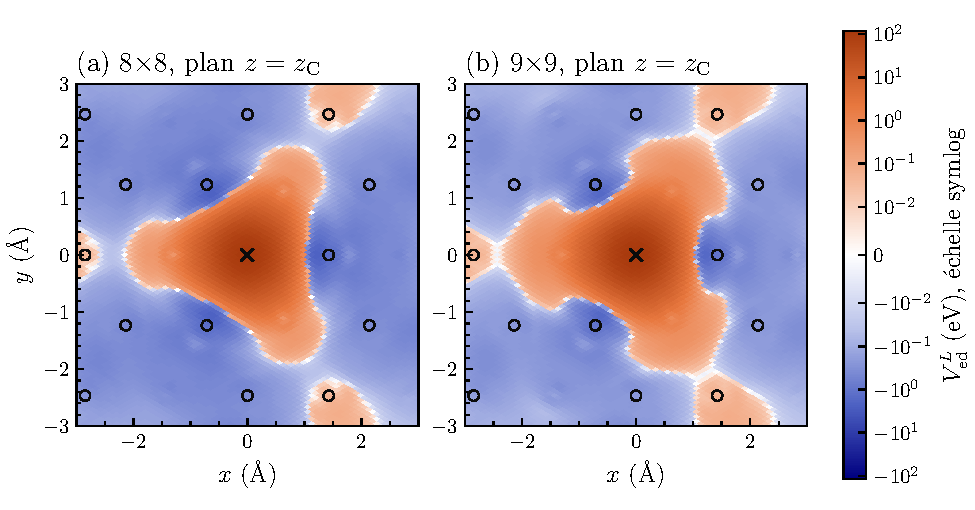
\includegraphics[width=\textwidth]{figures/fig_Ved_zoom.pdf}
    \caption[Potentiel de défaut local au voisinage de la lacune pour deux tailles de super-cellule.]{Potentiel de défaut local $V_\text{ed}^\text{L}$ dans le plan du graphène $(z=z_\text{C})$ au voisinage de la lacune, représentée par une croix, pour les super-cellules (a) $8\times 8$ et (b) $9\times 9$. L'échelle est symétrique logarithmique et linéaire entre $\pm 10^{-2}$~eV. Nous voyons une différence qualitative de la forme et de l'orientation des lobes du potentiel de défaut entre les deux tailles de super-cellules. Les deux super-cellules partagent les paramètres de calcul et la
    géométrie non relaxée décrits dans cette section ; seule la divisibilité de la taille $N$ par trois, et donc l'inclusion ou non des points $K$ et $K'$ dans l'échantillonnage, les distingue.}
    \label{fig:Ved_zoom}
\end{figure}

D'abord, la troisième colonne du tableau~\ref{tab:échantillonnage} montre le déplacement du niveau de Fermi $\Delta E_F$ à la création de la lacune. Avec la troncature de Coulomb bidimensionnelle, les super-cellules parfaite et défectueuse ont un zéro d'énergie commun : le décalage dans le vide, mesuré dans le bloc \og Alignement du potentiel \fg{} dans cette section. Nous y trouvons un décalage nul à quelques meV près (nul à un ou deux écarts-types près). Pour la famille qui inclut les points $K$ et $K'$, le déplacement $\Delta E_F$ est de cet ordre, donc compatible avec zéro. Les tailles de l'autre famille présentent systématiquement des déplacements de quelques centaines de meV, ce qui signale qu'il y a bien une différence physique. Un autre indice se trouve dans la quatrième colonne, qui rapporte la moyenne $\bar V_\text{ed}^{\text{L}}(a_\text{CC})$ du potentiel autour de la lacune. Les deux familles se distinguent par l'ordre de grandeur et le signe. Enfin, la figure~\ref{fig:Ved_zoom} présente des différences qualitatives entre la forme et l'orientation du potentiel de défaut local de la lacune.

Toutes les super-cellules partagent les mêmes paramètres de calcul et la même géométrie non relaxée (hormis la position exacte du défaut). Seule la divisibilité de la taille $N$ par trois, et donc l'inclusion ou non des points $K$ et $K'$ dans l'échantillonnage, les distingue. Ainsi, nous ne retenons que la famille incluant les points $K$ et $K'$, dont la super-cellule $9\times 9$ sert de référence et les $6\times 6$ et $12\times 12$ servent de contrôle de convergence. L'autre famille, qui n'inclut pas les points $K$ et $K'$, est conservée comme contrôle des artefacts d'échantillonnage.

\bigskip
\bloc{Remplissage par zéros}

Nous vérifions ici la validité de la technique de remplissage par zéros. La figure~\ref{fig:Ved} (a,b) montre le potentiel de lacune local dans le plan du graphène pour les super-cellules $5\times 5$ et $9\times 9$ et (c) montre sa moyenne dans le plan, excluant un rayon de $0.5$~\AA{} autour de chaque atome où la réorganisation autocohérente de la densité de charge rend le potentiel abrupt et la moyenne sensible à la grille, en fonction de la distance au site de la lacune pour les six tailles. Le site de la lacune, dépourvu d'atome, n'est pas exclu de cette moyenne.

\begin{figure}[htbp]
    \centering
    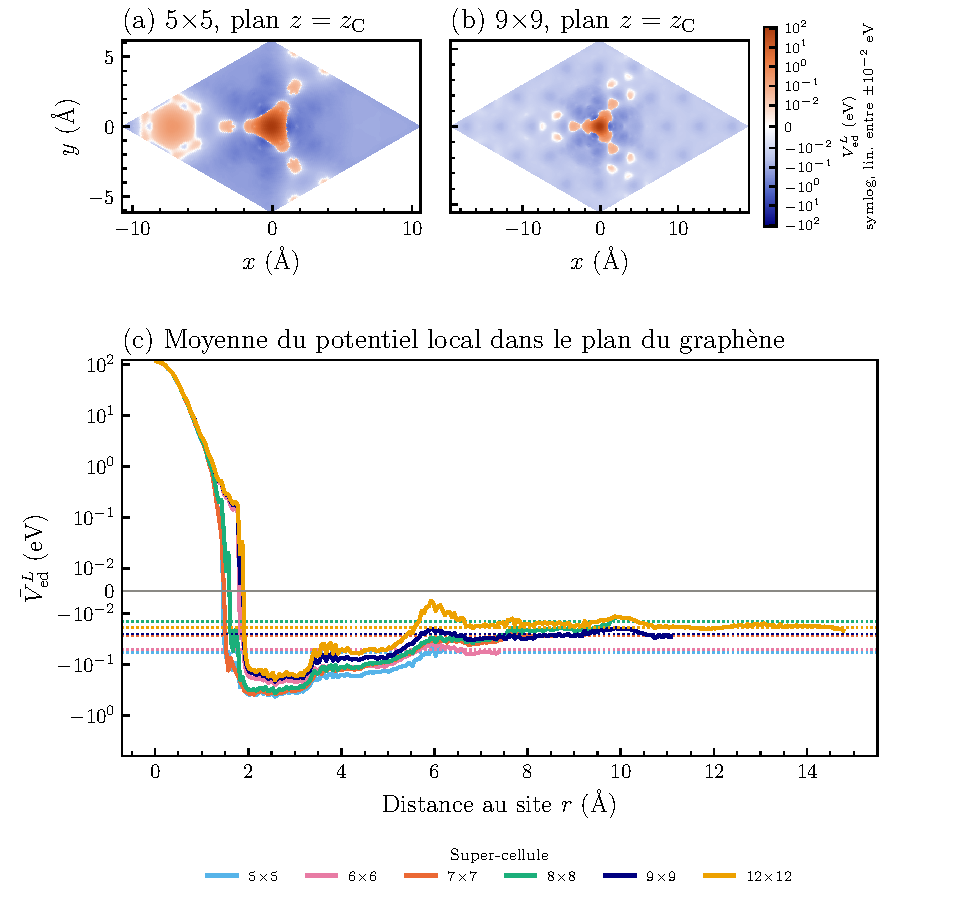
\includegraphics[width=\textwidth]{figures/fig_Ved.pdf}
    \caption[Potentiel de lacune local dans le graphène.]{Potentiel local $V_\text{ed}^\text{L}$ de la lacune. (a,b) Dans le plan du graphène ($z=z_\text{C}$), pour les super-cellules $5\times 5$ et $9\times 9$ avec une échelle de couleur symétrique logarithmique, linéaire entre $\pm 10^{-2}$~eV. Notons la zone positive autour de l'atome le plus éloigné de la lacune en (a), absente en (b), qui représente l'interaction de la lacune avec ses images périodiques. (c) Moyenne du potentiel local dans le plan du graphène $\bar V_\text{ed}^\text{L}$, excluant un rayon de $r_\text{at} = 0.5$~\AA{} autour des c\oe urs atomiques, pour les six tailles de super-cellules. Les traits pointillés horizontaux marquent la constante d'alignement $\Delta V_\text{PA}^{(N)}$ de chaque taille. Chaque courbe s'arrête à la demi-largeur de la super-cellule, soit le rayon du cercle inscrit dans la cellule de Wigner-Seitz centrée sur la lacune.}
    \label{fig:Ved}
\end{figure}

Le potentiel de la lacune est dominé par un c\oe ur positif répulsif de l'ordre de $115$ à $116$~eV au site de la lacune, où manque le c\oe ur attractif de l'atome supprimé. Le potentiel chute ensuite de trois ordres de grandeur en moins de $2$~\AA{}. Toutefois, il ne s'annule pas : un fond négatif faible subsiste jusqu'à la frontière, de $-0.1$~eV pour $N=5$ à $-0.018$~eV pour $N=12$. Ce fond est uniforme et coïncide, à $6$~meV près pour $N\geq 6$, avec la constante d'alignement $\Delta V_\text{PA}^{(N)}$ de la section~\ref{sec:M_détails}, tracée en pointillés au panneau (c). Nous discutons de sa nature au bloc suivant. Seule la super-cellule $N=5$ fait exception. Son fond s'écarte de $\Delta V_\text{PA}^{(5)}$ d'une quarantaine de meV. De plus, le panneau (a) montre une zone positive autour de l'atome le plus éloigné de la lacune, au sommet de la cellule de Wigner-Seitz, équidistant de la lacune elle-même et de deux de ses images. Cette zone, absente du panneau (b), est le signe de l'interaction de la lacune avec ses propres images~\cite{freysoldtFirstprinciplesCalculationsPoint2014}. La super-cellule $N=5$ est trop petite pour contenir la lacune, tandis que la $N=9$ est suffisante.

Le remplissage par zéros impose $V_\text{ed}^\text{L} = 0$ au-delà de la frontière, où le fond, quoique faible, ne s'annule pas encore. Le potentiel élargi présente alors une discontinuité de $10^{-2}$ à $10^{-1}$~eV à la frontière. Trois facteurs bornent cette approximation. D'abord, la discontinuité est trois ordres de grandeur sous le c\oe ur de la lacune qui domine le couplage. Ensuite, comme le fond vaut la constante d'alignement et que remplissage et alignement commutent (section~\ref{sec:M_détails}), le potentiel aligné et élargi n'a plus à la frontière que l'écart entre le fond et $\Delta V_\text{PA}^{(N)}$, inférieur à $6$~meV pour $N\geq 6$. Enfin, deux vérifications indépendantes bornent l'erreur sur la matrice elle-même : la convention intensive, plus loin, montre que le remplissage préserve l'échelle de $\bm M$ à mieux que $2.4~\%$ pour $N\geq 7$ et la localisation dans la base de Wannier montre qu'il est indispensable à l'interpolation. C'est une approximation maîtrisée, dont l'erreur est bornée.

\bigskip
\bloc{Alignement du potentiel}

Malgré la troncature de Coulomb bidimensionnelle qui est supposée aligner la référence des deux calculs de super-cellules avec le vide, nous trouvons tout de même un décalage uniforme loin de la lacune dans le plan. Le tableau~\ref{tab:alignement} quantifie ce décalage pour diverses tailles de super-cellules et divers schémas de calcul.

\begin{table}[htbp]
    \centering\small
    \caption[Constantes d'alignement selon quatre schémas et décalage du vide.]{Constantes d'alignement dans le plan du potentiel de la lacune selon quatre prescriptions et décalage du vide. La constante d'alignement est la moyenne des potentiels (sphères de $1$~\AA) sur (A) les sites à $d\geq0.75\,r_\text{max}$ (notre schéma), (B) les sites hors du cercle inscrit dans la cellule de Wigner-Seitz autour de la lacune de rayon $N a/2$ (Kumagai-Oba 2D), (C) les sites hors de la sphère inscrite dans la cellule de Wigner-Seitz de rayon $\min(Na/2, c/2)$ (Kumagai-Oba 3D) et (D) le site unique le plus éloigné de la lacune (Lu \textit{et al.}~\cite{luEfficientInitioCalculations2019}). L'écart-type des sites donne l'incertitude. (E) Décalage du vide : moyenne et écart-type pour $5\leq|z|\leq c/2=7.9$~\AA. Toutes les valeurs en meV.}
    \label{tab:alignement}
    \begin{tabular}{c r r r r r}
    \hline\hline
    $N$ & (A) Nous & (B) Kumagai-Oba 2D & (C) Kumagai-Oba 3D & (D) Lu \textit{et al.} & (E) Vide \\
    \hline
    5  & $-57.6 \pm 94.1$ & $-38.6 \pm 99.8$ & $-38.6 \pm 99.8$ & $-122.3$ & $-10.9 \pm 9.8$ \\
    6  & $-50.5 \pm 24.6$ & $-71.0 \pm 24.4$ & $-71.0 \pm 24.4$ & $-98.6$  & $-16.2 \pm 20.4$ \\
    7  & $-26.9 \pm 18.5$ & $-24.6 \pm 17.9$ & $-22.1 \pm 20.8$ & $-38.5$  & $-4.9 \pm 4.3$ \\
    8  & $-14.4 \pm 18.9$ & $-13.5 \pm 21.4$ & $-14.4 \pm 18.9$ & $-23.0$  & $-5.3 \pm 5.3$ \\
    9  & $-25.1 \pm 9.1$  & $-31.7 \pm 10.9$ & $-25.0 \pm 9.5$  & $-24.7$  & $-7.0 \pm 8.7$ \\
    10 & $-9.3 \pm 6.1$   & $-9.0 \pm 5.7$   & $-10.2 \pm 7.2$  & $-8.2$   & $-3.2 \pm 3.0$ \\
    11 & $-9.6 \pm 5.8$   & $-7.6 \pm 6.5$   & $-10.4 \pm 6.8$  & $-12.2$  & $-3.0 \pm 3.1$ \\
    12 & $-18.7 \pm 5.4$  & $-20.5 \pm 6.2$  & $-17.4 \pm 6.0$  & $-29.2$  & $-3.7 \pm 4.5$ \\
    \hline
    15 & $-16.2 \pm 2.8$  & $-17.8 \pm 3.1$  & $-13.4 \pm 5.5$  & $-15.6$  & $-7.1 \pm 8.6$ \\
    21 & $-14.2 \pm 1.0$  & $-14.7 \pm 1.0$  & $-8.8 \pm 7.9$   & $-13.8$  & $-2.6 \pm 1.4$ \\
    \hline\hline
\end{tabular}

\end{table}

Les deuxième et troisième colonnes comparent notre schéma (A) à celui de Kumagai-Oba~\cite{kumagaiElectrostaticsbasedFinitesizeCorrections2014} transposé en deux dimensions. Les deux prescriptions donnent les mêmes constantes à un ou deux écarts-types près (pour $N\geq 7$) ; la seule différence est que notre schéma retient deux à trois fois plus de sites, donnant une plus petite erreur statistique. La quatrième colonne montre le schéma Kumagai-Oba original où la région est bornée par $c/2$ dès $N\geq 7$ et inclut la queue du potentiel près de la lacune : il ne convient pas en 2D et nous l'ignorons pour la suite. La cinquième colonne montre le potentiel à un site de Lu \textit{et al.}~\cite{luEfficientInitioCalculations2019}, qui fluctue avec le site choisi. Parmi ces schémas, nous ne retenons que le nôtre (A). Enfin, la dernière colonne montre le décalage du vide, que nous mesurons dans la région entre $|z|=5$ et $|z|=c/2=7.9$~\AA{} et l'incertitude statistique est l'écart-type de ce décalage sur les points dans cette région. Nous trouvons un décalage presque nul (nul à un ou deux écarts-types près) et nous nous attendons à ce qu'une mesure plus propre, en moyennant plan par plan le potentiel électrostatique seulement (sans la contribution d'échange-corrélation) dans un vide plus épais, puisse rapprocher ce résidu de zéro.

Idéalement, la constante d'alignement devrait converger en taille de la super-cellule vers le décalage du vide. Notre schéma ne le fait pas (B et D non plus) : il semble converger vers une constante non nulle. Seul le (C) semble le faire, mais nous devons l'écarter pour la raison mentionnée plus haut. Il n'est pas tout à fait clair quelle référence, entre celle de la constante d'alignement dans le plan et celle du vide, est la bonne. Nous retenons alors les deux et examinons leurs conséquences sur le reste de ce chapitre et le suivant. Nous appelons \og aligné \fg{} notre schéma dans le plan et \og brut \fg{} le schéma où la référence est le décalage du vide.

Cette différence est toutefois surprenante et nous ne pouvons pas établir son origine.
Il est possible que la différence tienne à la comparaison des deux références et non la physique de la lacune. Pour (A), un test pourrait être de mesurer la constante pour différents rayons de sphères ou pour des sphères centrées sur des points interstitiels. Pour (E), mesurer le profil planaire $\Delta \bar V(z)$ sur toute la hauteur de la boîte montrerait s'il y a une marche entre le plan et le vide. Nous notons aussi qu'à taille comparable, l'écart entre le plan et le vide est environ deux fois plus faible, pour $N\geq 8$ et à la limite de l'incertitude statistique, pour la famille qui n'échantillonne pas $K$ ($N\neq 3m$), ce qui laisse supposer que l'échantillonnage proche de ce point est une cause plausible. Au seul point $\Gamma$, les super-cellules $N=3m$ placent huit états exactement au point de Dirac ($K$ et $K'$, bandes $\pi$ et $\pi^*$, deux spins), ce qui surestime la densité d'états du cône dans la fenêtre d'élargissement et pourrait faciliter un transfert de charge entre les états induits par la lacune et ces états étendus. La lacune porterait alors une charge effective qui lui donnerait une composante de longue portée à son potentiel. Des calculs de super-cellules avec un échantillonnage $\kv$ plus dense, non seulement à $\Gamma$, sont requis pour établir son origine.

\bigskip
\bloc{Convention intensive}

Nous vérifions ici la convention intensive de la section~\ref{sec:M_détails} : les éléments de matrice, calculés avec les états de Bloch normalisés sur la cellule unitaire, doivent être indépendants de la taille $N$. Nous le faisons sur les parties locale et non locale, puis sur la matrice complète. Le tableau~\ref{tab:L_NL} donne, pour les deux parties, la demi-trace de la paire dégénérée $(\pi,\pi^*)$ au point de Dirac,
\begin{equation}
    \bar M^\text{X}(K) = \tfrac{1}{2}\,\mathrm{Re}\,\mathrm{Tr}\,M^\text{X}(K,K),\qquad \text{X}=\text{L},\,\text{NL},\label{eqn:M_bar}
\end{equation}
invariante, comme la norme, sous les rotations unitaires de la paire. La partie non locale est constante à $10^{-3}$~eV près ; elle ne dépend ni de la taille ni de l'alignement, puisqu'elle est simplement le retrait des projecteurs de Kleinman-Bylander de l'atome absent et ne touche pas au potentiel. La partie locale brute est constante à l'intérieur de chaque famille et nous attribuons l'écart de $7~\%$ entre les deux familles à la différence physique d'échantillonnage. Les deux parties brutes sont donc intensives. La partie locale domine le couplage : elle porte $77$ à $79~\%$ de $\bar M(K)$ pour les matrices brutes et $79$ à $82~\%$ pour les matrices alignées. Sur toute la zone, le rapport des normes de Frobenius $\langle\|\bm M^\text{NL}\|\rangle/\langle\|\bm M^\text{L}\|\rangle$ vaut $0.25$ à $0.26$, brut comme aligné. Cette séparation n'a pas de sens physique en soi car elle dépend de notre choix de pseudo-potentiels.

\begin{table}[htbp]
    \centering
    \caption[Contributions locale et non locale
     à la matrice de couplage électron-défaut.]{Demi-trace invariante $\bar M^\text{X}(K)$ de l'équation~\eqref{eqn:M_bar} des parties locale (X=L) brute et alignée et non locale (X=NL) au point de Dirac $K$ pour les six tailles, en eV. La quatrième colonne donne le terme d'alignement $N^2|\Delta V_\text{PA}^{(N)}|$, égal à la différence des colonnes alignées et brutes. Pour $N=5, 7, 8$, dont les grilles élargies ne contiennent pas $K$, le point de la grille le plus proche est utilisé.}
    \label{tab:L_NL}
    % Généré par scripts/make_tables.py : ne pas éditer (python scripts/make_tables.py --only L_NL).
% tab:L_NL, §4.1.6, corps. Valeurs et sources cellule par cellule : tables/SOURCES.md.
% Sources : M2_plateau/M_analysis.npz ; M2_plateau/lnl_frobenius.csv
\begin{tabular}{c c c c c c}
    \hline\hline
    & \multicolumn{2}{c}{$\bar M^\text{L}(K)$ (eV)} & $\bar M^\text{NL}(K)$ & \multicolumn{2}{c}{NL/L toute la BZ} \\
    \cline{2-3}\cline{5-6}
    $N$ & brut & aligné & (eV) & brut & aligné \\
    \hline
    5  & $10.534$ & $11.973$ & $3.100$ & $0.258$ & $0.257$ \\
    6  & $11.356$ & $13.174$ & $3.103$ & $0.252$ & $0.252$ \\
    7  & $10.486$ & $11.805$ & $3.101$ & $0.258$ & $0.258$ \\
    8  & $10.734$ & $11.657$ & $3.101$ & $0.257$ & $0.257$ \\
    9  & $11.305$ & $13.342$ & $3.103$ & $0.252$ & $0.252$ \\
    12 & $11.222$ & $13.913$ & $3.103$ & $0.252$ & $0.252$ \\
    \hline\hline
\end{tabular}

\end{table}

La figure~\ref{fig:M_scaling} étend ce test à la matrice complète en comparant le maximum de $|M|$ sur toutes les bandes et toutes les paires $(\kv',\kv)$, en fonction de $N$, d'une part sur les grilles élargies $pN\times pN$ (cercles) et d'autre part sur les grilles grossières $N\times N$ (croix). Pour les grilles élargies, le maximum varie de $2.3~\%$ pour la famille $N=3m$ et de $2.1~\%$ pour $N\neq 3m$. La dispersion de $7.7~\%$ sur les six tailles est encore la manifestation de l'écart entre les deux familles. De plus, pour $N\geq 7$, l'écart entre les grilles grossières et élargies est inférieur à $2.4~\%$, ce qui confirme que le remplissage par zéros préserve l'échelle des matrices. L'écart résiduel à $N=5$ et $6$ s'explique par le fait que ces deux tailles sont trop petites pour contenir le potentiel, comme à la figure~\ref{fig:Ved}~(a), et leur remplissage par zéros diffère réellement de leur prolongement périodique.

\begin{figure}[htbp]
    \centering
    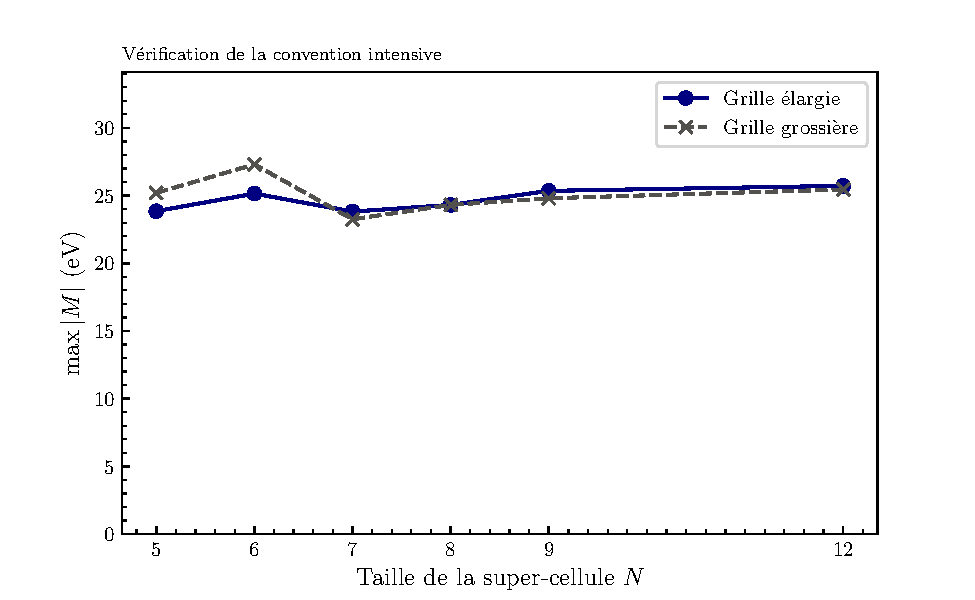
\includegraphics[width=\textwidth]{figures/fig_M_scaling_final.pdf}
    \caption[Vérification de la convention intensive des éléments de matrice.]{Maximum de $|M|$ sur toutes les bandes et toutes les paires $(\kv',\kv)$ en fonction de la taille $N$ de la super-cellule. Les croix représentent les grilles grossières tandis que les cercles représentent les grilles élargies ; les matrices sont les matrices brutes (section~\ref{sec:M_détails}). L'indépendance en $N$ vérifie la convention intensive de la section~\ref{sec:M_détails}. L'écart à $N=5$ et $6$ entre les deux types de grilles correspond aux super-cellules qui ne contiennent pas entièrement le potentiel de défaut (figure~\ref{fig:Ved} (a)). Le maximum est atteint hors de $\kv'=\kv$ et ne dépend pas de l'alignement.}
    \label{fig:M_scaling}
\end{figure}

Ces deux tests portent sur les matrices brutes. Pour les matrices alignées, le retranchement de $\Delta V_\text{PA}^{(N)}$ sur les $N^2$ cellules ajoute à $\bm M$ le terme $-\Delta V_\text{PA}^{(N)}S(\kv'-\kv)$. En $\kv'=\kv$, ce terme vaut exactement $N^2|\Delta V_\text{PA}^{(N)}|$, ce que les colonnes brutes et alignées du tableau~\ref{tab:L_NL} vérifient : il croît comme $N^2$ et la matrice alignée n'est pas intensive pour ces points. Pour $\kv'\neq \kv$, le facteur de forme $S$ l'étale sur les points de la grille élargie voisins de $\kv'=\kv$ et s'annule sur les autres points de la grille grossière. Le maximum de $|M|$, atteint hors de $\kv'=\kv$, ne change pas avec l'alignement (au plus $0.8~\%$ pour $N=5$) : la figure ne peut pas tester cette composante. Seuls la composante $\kv'=\kv$ et son étalement par $S$, fixés par l'alignement, échappent à la convention intensive. Cet effet est réduit par la troncature : il ne reste que $-\Delta V_\text{PA}^{(N)}$ sur les cellules retenues. Nous mesurons cet effet sur le taux d'amortissement à la section~\ref{sec:T_results}.

\newpage
\bloc{Éléments de matrice au point de Dirac et comparaison avec la littérature}

La figure~\ref{fig:kaasbjerg_M} caractérise le couplage depuis le voisinage du point de Dirac, où résident les états pertinents pour la diffusion Raman résonante. Au point $K$, les bandes $\pi$ et $\pi^*$ sont dégénérées et un élément de matrice individuel n'est pas défini de manière unique. Nous suivons Kaasbjerg~\cite{kaasbjergAtomisticMatrixTheory2020} et fixons l'état initial à $\kv=K+\delta\hat{\mathbf{x}}$, légèrement décalé de $K$, puis traçons l'élément intrabande $A_\text{cell}|M_{nn}(\kv',\kv)|$ pour $n=\pi$ et $\pi^*$, et pour l'état final $\kv'$ parcourant la zone de Brillouin sur une grille de sortie $240\times 240$. Nous le faisons pour les deux références : les matrices brutes (a,b) et alignées (c,d). Le facteur $A_\text{cell}=5.27$~\AA$^2$ est l'aire de la cellule unitaire et donne des éléments en eV\,\AA$^{2}$. Les variantes brutes et alignées ne diffèrent qu'au voisinage de $K$, où le terme $N^2|\Delta V_\text{PA}^{(N)}|$ du bloc précédent, étalé par le facteur de forme, augmente les éléments de quelques eV\,\AA$^2$. Elles coïncident partout ailleurs, en particulier autour de $K'$.

Kaasbjerg rapporte environ $70$~eV\,\AA$^2$ pour les éléments intravallée $\pi$ d'une lacune dans le graphène et environ $80$~eV\,\AA$^2$ pour $\pi^*$ ; la première est écrite dans son texte, la seconde se lit sur la barre de couleur de sa figure~3. Notre figure~\ref{fig:kaasbjerg_M} reproduit la grandeur. Son calcul emploie le formalisme PAW qui reconstruit les fonctions d'onde tous-électrons à partir d'un calcul à c\oe urs gelés dans le code \texttt{GPAW}, la fonctionnelle LDA et une super-cellule $11\times 11$. Il impose au potentiel de s'annuler aux bords de la cellule hors du plan. Cela correspond à nos matrices brutes des panneaux (a,b), qui se comparent à convention égale. L'article indique que la relaxation structurelle, mineure pour les défauts de dichalcogénures, est négligée, mais ne précise pas si ce choix s'étend au graphène, où la reconstruction autour de la lacune n'est pas vraiment mineure. Sa convention intensive est identique à la nôtre et l'interprétation physique concorde : il attribue, comme nous, le signe répulsif au c\oe ur attractif manquant de l'atome supprimé.

Près de $K$, en moyennant sur un disque de $0.15$~\AA$^{-1}$, nos éléments valent $77.0$ ($\pi$) et $78.2$ ($\pi^*$)~eV\,\AA$^{2}$ pour les matrices brutes et $81.6$ ($\pi$) et $82.8$~eV\,\AA$^{2}$ ($\pi^*$) pour les matrices alignées. Près de $K'$, nous trouvons $81.2$ ($\pi$) et $82.3$~eV\,\AA$^2$ ($\pi^*$) dans les deux cas. Nous sommes donc à $10$~\% ($\pi$) au-dessus et $2.3$~\% ($\pi^*$) en dessous de Kaasbjerg, pour les matrices brutes à convention égale. Un écart de cet ordre est celui qu'on attend des différences de méthode : PBE contre LDA, pseudo-potentiels ONCV contre PAW, super-cellule $9\times 9$ contre $11\times 11$ et ondes planes contre orbitales atomiques. De plus, nous n'avons pas sa valeur exacte pour $\pi^*$ : nous la déduisons de la barre de couleur. Nous ne chercherons pas à attribuer cette différence à une de ces causes : les éléments de matrice sont des quantités intermédiaires qui dépendent du formalisme. La comparaison probante se fait au niveau des observables, le taux d'amortissement et la densité d'états, à la section~\ref{sec:T_results} du chapitre suivant.


\clearpage
\vspace*{\fill}
\begin{figure}[htbp]
    \centering
    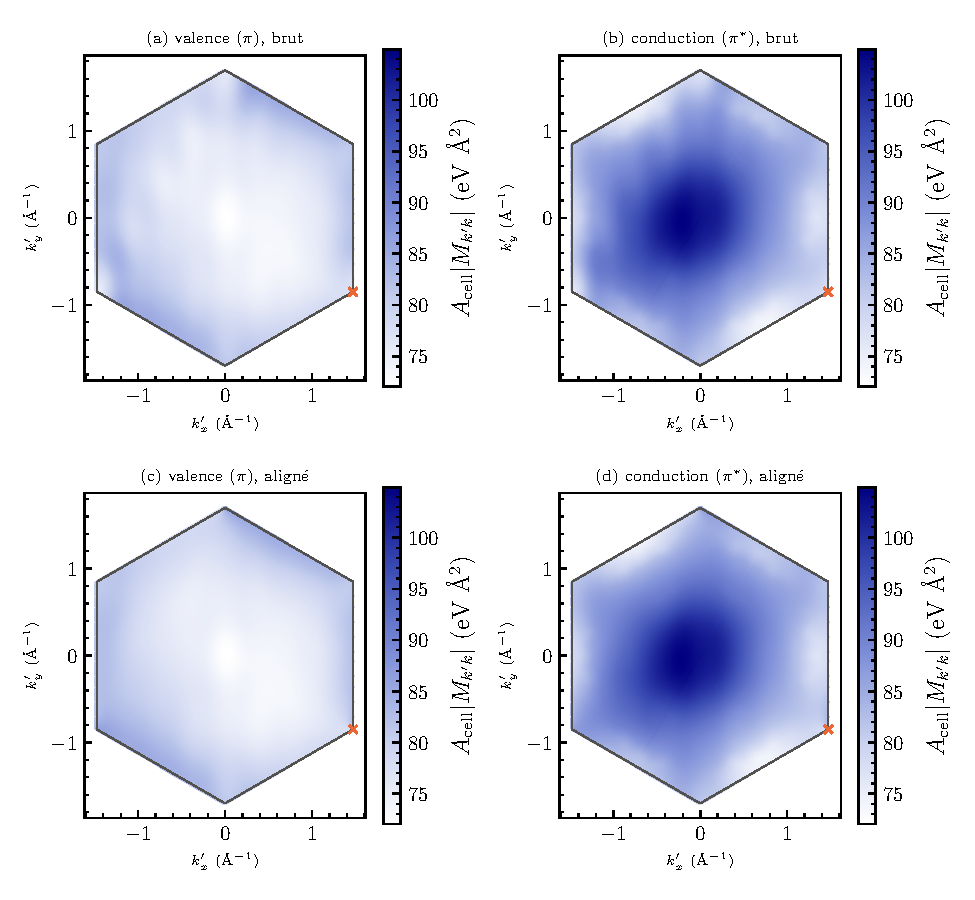
\includegraphics[width=\textwidth]{figures/fig_kaasbjerg_plateau_ws.pdf}
    \caption[Élément de matrice intrabande depuis le voisinage du point de Dirac.]{Élément de matrice intrabande $A_\text{cell}|M_{nn}(\kv',\kv)|$ depuis l'état initial $\kv = K+\delta\hat{\bm x}$ (croix), légèrement décalé de $K$ pour contourner la dégénérescence, vers $\kv'$ sur une grille de sortie $240\times240$, pour $n=\pi$ (valence) et $n=\pi^*$ (conduction) et une super-cellule $9\times 9$. (a,b) Matrices brutes. (c,d) Matrices alignées. C'est la grandeur tracée à la figure~3 de Kaasbjerg~\cite{kaasbjergAtomisticMatrixTheory2020}.}
    \label{fig:kaasbjerg_M}
\end{figure}
\vspace*{\fill}
\clearpage

\bloc{Localisation dans la base de Wannier}

La figure~\ref{fig:M_locality} présente la norme de Frobenius des blocs $M_{ij}(\Rv,\bm 0)$ en fonction de la distance $R$ à la lacune située à l'origine après le recentrage, pour les quatre super-cellules $N=5, 8, 9, 12$ sur la grille élargie obtenue par remplissage par zéros et, pour $N=5, 8$, sur la grille grossière $N\times N$.

\begin{figure}[htbp]
    \centering
    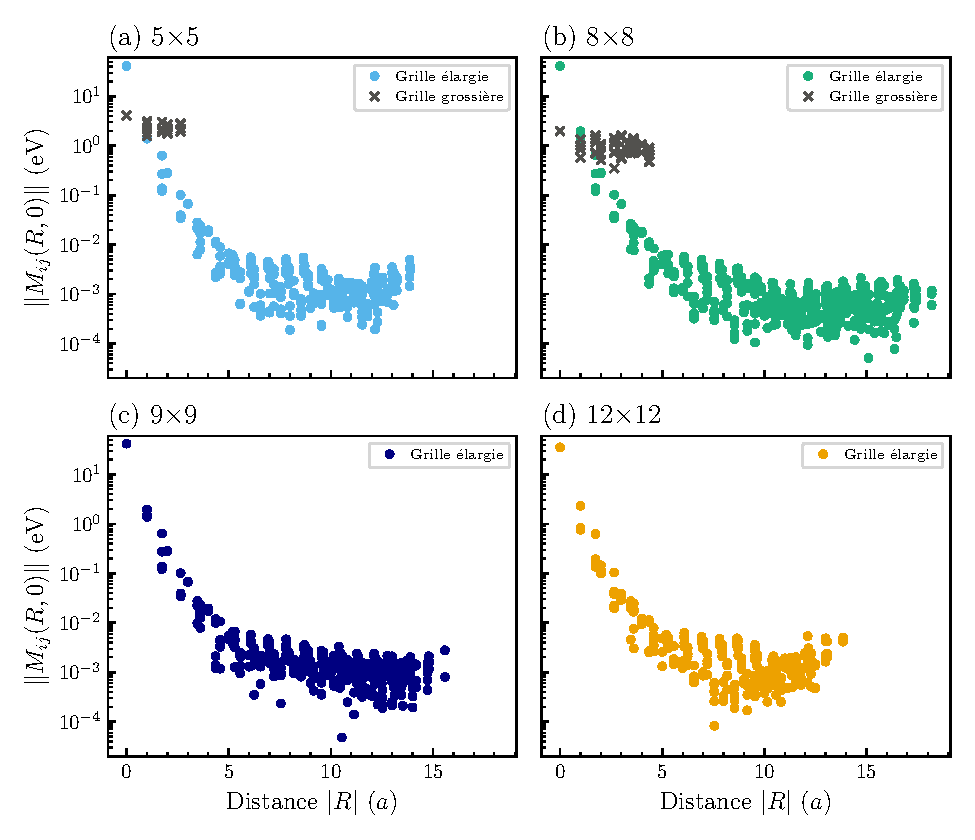
\includegraphics[width=\textwidth]{figures/fig_locality_final.pdf}
    \caption[Localisation de la matrice de couplage électron-lacune dans la base des fonctions de Wannier.]{Norme de Frobenius des blocs $M_{ij}(\Rv,\bm 0)$ de la matrice de couplage électron-lacune dans la base des fonctions de Wannier, où la lacune a été ramenée à l'origine par recentrage, en fonction de
    la distance $R$ en unités du paramètre de maille, pour les
    super-cellules $N = 5, 8, 9, 12$. Les cercles représentent les grilles élargies $pN\times pN$ et les croix identifient les grilles grossières $N\times N$ (a,b). Les normes hors site ne dépendent pas de la référence : l'alignement ne modifie que le bloc sur site $(\bm 0,\bm 0)$.}
    \label{fig:M_locality}
\end{figure}

D'une part, les grilles grossières (croix aux panneaux (a,b)) ne donnent pas lieu à une décroissance rapide. D'autre part, sur les grilles élargies (cercles), le poids chute de plus de trois ordres de grandeur sur les cinq premières cellules unitaires avant d'atteindre un plancher de $10^{-3}$~eV. C'est la décroissance rapide attendue des éléments de matrice dans la base des fonctions de Wannier pour un défaut localisé dans l'espace réel. Cette différence entre les deux types de grilles est un effet de repliement spectral (de l'anglais \textit{aliasing}). La transformée~\eqref{eqn:M_wannier} sur une grille de $N\times N$ points ne produit que $N^2$ vecteurs $\Rv$ et tout poids situé au-delà de cette boîte est replié sur les mailles disponibles, ce qui étale artificiellement le poids et masque la localisation. Les grilles élargies de $pN\times pN$ points disposent de $p^2$ fois plus de vecteurs $\Rv$ et rendent la localisation manifeste. Le remplissage par zéros est donc indispensable à l'interpolation de Wannier : sans lui, la représentation réelle du couplage n'est pas localisée et aucune troncature n'est légitime.

Le tableau~\ref{tab:rcut_M} de l'annexe~\ref{annexe:M} mesure l'effet de la troncature sur les éléments de matrice interpolés, pour les deux références. À $R_\text{cut} =3$ (norme euclidienne des indices réduits), soit 29 cellules unitaires, l'écart aux éléments de matrice obtenus avec toutes les mailles est de $1.7$ à $3.3~\%$ pour les matrices alignées, mais de $7$ à $12~\%$ pour les matrices brutes. Dans les deux cas, la décroissance ralentit au-delà et l'écart plafonne autour de $1~\%$ à $R_\text{cut}=6$ (113 cellules). Cet écart résiduel est la contribution cumulée des centaines de cellules restantes de la boîte, dont la norme individuelle est au plancher de $10^{-3}$~eV de la figure~\ref{fig:M_locality}. L'écart entre les deux références est porté par les blocs diagonaux $M_{ij}(\Rv,\Rv)$, les seuls modifiés par l'alignement, et sa grandeur est celle du terme $(N^2-29)|\Delta V_\text{PA}^{(N)}|$ rapporté à $\max|M|$ : $5~\%$ pour $9\times 9$ et $8~\%$ pour $12\times 12$. C'est la même composante $\kv'=\kv$ qu'au bloc \og Convention intensive \fg{}. Nous retenons $R_\text{cut}=3$ pour la production et la section~\ref{sec:T_results} vérifie ce que ces écarts deviennent sur le taux d'amortissement, pour les deux références.

\bigskip
\bloc{Autres vérifications}

Les vérifications de la chaîne de calcul de la matrice $\bm M$ sont rassemblées au tableau~\ref{tab:tests_M} de l'annexe~\ref{annexe:M}. La plus contraignante applique la machinerie au potentiel de Kohn-Sham de la super-cellule parfaite et reconstruit les valeurs propres de \texttt{QuantumESPRESSO} à $1.5$--$32~\mu$eV près sur les grilles grossières (figure~\ref{fig:ks_reconstruction}). Elle valide, contre une référence indépendante du code, tout ce qui précède la soustraction des deux super-cellules. L'application directe du potentiel de la lacune aux états de Bloch repliés, sans passer par la chaîne, reproduit $\bm M^\text{L}/N_\text{cells}$ et $\bm M^\text{NL}$ à $10^{-14}$~eV sur les grilles grossières et à $10^{-8}$~eV sur les grilles élargies. Ce test fixe la normalisation de la section~\ref{sec:M_détails}, en particulier le facteur $N^2$ qui ramène la partie locale à la cellule unitaire. Les autres tests (hermiticité, remplissage, transformées aller-retour) sont au niveau du bruit numérique, $10^{-14}$ à $10^{-15}$. Le seul écart supérieur, $10^{-3}$ entre grilles grossières et grilles élargies aux points $\kv$ communs, vient de la différence des deux densités autocohérentes et non de la chaîne de calcul.

\section{Conclusion}

Ce chapitre a construit, à partir des premiers principes, la matrice de couplage électron-défaut $\bm M$ qui entre directement dans les amplitudes \textit{phonon-défaut} du chapitre~\ref{chap:Raman}. Les éléments de matrice sont définis à partir du potentiel induit par le défaut, séparés en une partie locale évaluée dans l'espace réciproque~\eqref{eqn:ML_final} et une partie non locale issue des projecteurs de Kleinman-Bylander~\eqref{eqn:MNL_final}, puis interpolés par fonctions de Wannier. Deux idées rendent la méthode praticable : le remplissage par zéros, qui raffine la grille du potentiel sans super-cellule démesurée et rend la localisation de $\bm M$ manifeste dans la base de Wannier, et la troncature de cette représentation à un sous-espace réduit, que le chapitre suivant exploite.

Appliquée à une lacune non relaxée dans le graphène, la méthode livre quatre résultats. L'échantillonnage au seul point $\Gamma$ sépare les super-cellules en deux familles selon qu'elles incluent ou non les points $K$ et $K'$. Nous retenons la famille $N=3m$, avec la super-cellule $9\times 9$ comme référence. Le potentiel de la lacune est un c\oe ur répulsif de $115$~eV qui chute de trois ordres de grandeur en moins de $2$~\AA, mais laisse un fond uniforme négatif, de $-0.1$~eV à $-18$~meV selon la taille, qui ne converge pas vers le décalage du vide. Faute d'en établir l'origine, nous conservons les deux références, les matrices brutes (référence du vide) et alignées (référence du plan), et suivons leurs conséquences jusqu'aux observables du prochain chapitre. La convention intensive est vérifiée sur les matrices brutes et l'alignement y ajoute un terme non intensif confiné à $\kv'=\kv$ et son voisinage. La partie locale porte $77$ à $82~\%$ du couplage au point de Dirac, et nos éléments intravallées près de $K$, $77$ et $78$~eV\,\AA$^2$ pour $\pi$ et $\pi^*$ pour les matrices brutes, se comparent à convention égale avec Kaasbjerg~\cite{kaasbjergAtomisticMatrixTheory2020}, à $10~\%$ près. La chaîne de calcul est validée contre une référence indépendante par la reconstruction des valeurs propres de Kohn-Sham à quelques dizaines de $\mu$eV près.

Ces résultats ont leurs limites. D'abord, la géométrie n'est pas relaxée et la reconstruction de Jahn-Teller de la monolacune~\cite{el-barbaryStructureEnergeticsVacancy2003} est ignorée. Les calculs ne sont pas polarisés en spin alors que la monolacune reconstruite porte un moment magnétique. Ensuite, les super-cellules ne sont échantillonnées qu'au point $\Gamma$, ce qui est à la fois la cause des deux familles et le suspect principal de l'asymptote non nulle de la constante d'alignement. Enfin, la bonne référence entre celle du vide et celle du plan reste indéterminée. Des calculs de super-cellules avec un échantillonnage plus dense que le seul point $\Gamma$ pourraient trancher la question sur les familles et l'origine de l'asymptote. D'autres tests de la référence, comme varier le rayon des sphères autour des sites retenus, déplacer les sphères à des sites interstitiels ou bien faire un profil du potentiel $\Delta\bar V(z)$ sur toute la boîte, pourraient également nous en apprendre plus sur l'origine du décalage entre les deux références.

Au terme de ce chapitre, nous disposons de la matrice de couplage électron-défaut $\bm M$, calculée \textit{ab initio} et tronquée dans la base de Wannier. Elle est l'élément constitutif du chapitre suivant qui la prend en entrée, pour les deux références, pour calculer la matrice $T$ et le taux d'amortissement $\Gamma$. C'est sur cette observable que l'effet de l'alignement et la comparaison avec la littérature se jugent.